\documentclass[twoside]{book}

% Packages required by doxygen
\usepackage{fixltx2e}
\usepackage{calc}
\usepackage{doxygen}
\usepackage{graphicx}
\usepackage[utf8]{inputenc}
\usepackage{makeidx}
\usepackage{multicol}
\usepackage{multirow}
\PassOptionsToPackage{warn}{textcomp}
\usepackage{textcomp}
\usepackage[nointegrals]{wasysym}
\usepackage[table]{xcolor}

% Font selection
\usepackage[T1]{fontenc}
\usepackage{mathptmx}
\usepackage[scaled=.90]{helvet}
\usepackage{courier}
\usepackage{amssymb}
\usepackage{sectsty}
\renewcommand{\familydefault}{\sfdefault}
\allsectionsfont{%
  \fontseries{bc}\selectfont%
  \color{darkgray}%
}
\renewcommand{\DoxyLabelFont}{%
  \fontseries{bc}\selectfont%
  \color{darkgray}%
}
\newcommand{\+}{\discretionary{\mbox{\scriptsize$\hookleftarrow$}}{}{}}

% Page & text layout
\usepackage{geometry}
\geometry{%
  a4paper,%
  top=2.5cm,%
  bottom=2.5cm,%
  left=2.5cm,%
  right=2.5cm%
}
\tolerance=750
\hfuzz=15pt
\hbadness=750
\setlength{\emergencystretch}{15pt}
\setlength{\parindent}{0cm}
\setlength{\parskip}{0.2cm}
\makeatletter
\renewcommand{\paragraph}{%
  \@startsection{paragraph}{4}{0ex}{-1.0ex}{1.0ex}{%
    \normalfont\normalsize\bfseries\SS@parafont%
  }%
}
\renewcommand{\subparagraph}{%
  \@startsection{subparagraph}{5}{0ex}{-1.0ex}{1.0ex}{%
    \normalfont\normalsize\bfseries\SS@subparafont%
  }%
}
\makeatother

% Headers & footers
\usepackage{fancyhdr}
\pagestyle{fancyplain}
\fancyhead[LE]{\fancyplain{}{\bfseries\thepage}}
\fancyhead[CE]{\fancyplain{}{}}
\fancyhead[RE]{\fancyplain{}{\bfseries\leftmark}}
\fancyhead[LO]{\fancyplain{}{\bfseries\rightmark}}
\fancyhead[CO]{\fancyplain{}{}}
\fancyhead[RO]{\fancyplain{}{\bfseries\thepage}}
\fancyfoot[LE]{\fancyplain{}{}}
\fancyfoot[CE]{\fancyplain{}{}}
\fancyfoot[RE]{\fancyplain{}{\bfseries\scriptsize Generated on Tue Nov 4 2014 20\+:13\+:18 for Aiki by Doxygen }}
\fancyfoot[LO]{\fancyplain{}{\bfseries\scriptsize Generated on Tue Nov 4 2014 20\+:13\+:18 for Aiki by Doxygen }}
\fancyfoot[CO]{\fancyplain{}{}}
\fancyfoot[RO]{\fancyplain{}{}}
\renewcommand{\footrulewidth}{0.4pt}
\renewcommand{\chaptermark}[1]{%
  \markboth{#1}{}%
}
\renewcommand{\sectionmark}[1]{%
  \markright{\thesection\ #1}%
}

% Indices & bibliography
\usepackage{natbib}
\usepackage[titles]{tocloft}
\setcounter{tocdepth}{3}
\setcounter{secnumdepth}{5}
\makeindex

% Hyperlinks (required, but should be loaded last)
\usepackage{ifpdf}
\ifpdf
  \usepackage[pdftex,pagebackref=true]{hyperref}
\else
  \usepackage[ps2pdf,pagebackref=true]{hyperref}
\fi
\hypersetup{%
  colorlinks=true,%
  linkcolor=blue,%
  citecolor=blue,%
  unicode%
}

% Custom commands
\newcommand{\clearemptydoublepage}{%
  \newpage{\pagestyle{empty}\cleardoublepage}%
}


%===== C O N T E N T S =====

\begin{document}

% Titlepage & ToC
\hypersetup{pageanchor=false,
             bookmarks=true,
             bookmarksnumbered=true,
             pdfencoding=unicode
            }
\pagenumbering{roman}
\begin{titlepage}
\vspace*{7cm}
\begin{center}%
{\Large Aiki }\\
\vspace*{1cm}
{\large Generated by Doxygen 1.8.8}\\
\vspace*{0.5cm}
{\small Tue Nov 4 2014 20:13:18}\\
\end{center}
\end{titlepage}
\clearemptydoublepage
\tableofcontents
\clearemptydoublepage
\pagenumbering{arabic}
\hypersetup{pageanchor=true}

%--- Begin generated contents ---
\chapter{readme}
\label{d7/d46/a00002}
\hypertarget{d7/d46/a00002}{}
\section*{Aiki }

The connecting scripting language Aiki. The scripting language was a school project but turned into~\newline
 a hobby exercise for compiler development. In the foreseeable future it will not be applicable on all ~\newline
 grounds in other terms of real world application, it was just a fun project.~\newline
~\newline
 Aiki aimed to be integrated easily with C++. The syntax is similar to that from Java. Unlike the language Java the Aiki is developed with ease of use from the command line while also utilizing precompiled binaries.

~\newline
 ~\newline
 \subsection*{Portability  Aiki will run on a several of platforms eventually. But for now it is only tested on Windows \& Linux. ~\newline
 It will probably work without and trouble on O\+S X. ~\newline
 ~\newline
  Contribution  Check out the issue tracker (or send me an e-\/mail, sometimes I am lazy with updating it) }
\chapter{Hierarchical Index}
\section{Class Hierarchy}
This inheritance list is sorted roughly, but not completely, alphabetically\+:\begin{DoxyCompactList}
\item \contentsline{section}{Environment}{\pageref{de/d21/a00006}}{}
\item \contentsline{section}{Fragment}{\pageref{d4/dee/a00008}}{}
\begin{DoxyCompactList}
\item \contentsline{section}{Expression}{\pageref{de/d5e/a00007}}{}
\item \contentsline{section}{Function\+Call}{\pageref{da/da0/a00009}}{}
\item \contentsline{section}{Function\+Definition}{\pageref{d7/dec/a00010}}{}
\item \contentsline{section}{Function\+Tail}{\pageref{df/d86/a00012}}{}
\item \contentsline{section}{Statement}{\pageref{d3/d52/a00023}}{}
\begin{DoxyCompactList}
\item \contentsline{section}{Assign\+Statement}{\pageref{d1/d7c/a00003}}{}
\item \contentsline{section}{If\+Statement}{\pageref{d7/dd4/a00013}}{}
\item \contentsline{section}{Return\+Statement}{\pageref{db/db2/a00020}}{}
\end{DoxyCompactList}
\end{DoxyCompactList}
\item \contentsline{section}{Function\+Signature}{\pageref{da/d45/a00011}}{}
\item \contentsline{section}{Intermediate\+Operation}{\pageref{d2/de7/a00014}}{}
\begin{DoxyCompactList}
\item \contentsline{section}{Byte\+Operation}{\pageref{d0/d0b/a00004}}{}
\item \contentsline{section}{Dword\+Operation}{\pageref{dd/dad/a00005}}{}
\begin{DoxyCompactList}
\item \contentsline{section}{Position\+Inquirer}{\pageref{d1/d2b/a00018}}{}
\end{DoxyCompactList}
\item \contentsline{section}{Position\+Reference}{\pageref{dd/da2/a00019}}{}
\end{DoxyCompactList}
\item \contentsline{section}{Operation\+Code}{\pageref{dd/d1b/a00015}}{}
\item \contentsline{section}{Operation\+Code\+Text}{\pageref{d7/d7a/a00016}}{}
\item \contentsline{section}{Parser}{\pageref{d4/d51/a00017}}{}
\item \contentsline{section}{Scope\+Type$<$ T $>$}{\pageref{de/d11/a00021}}{}
\item \contentsline{section}{Scope\+Type$<$ string $\ast$ $>$}{\pageref{de/d11/a00021}}{}
\item \contentsline{section}{Scope\+Type$<$ Variable $\ast$ $>$}{\pageref{de/d11/a00021}}{}
\item \contentsline{section}{Stack$<$ T $>$}{\pageref{d7/de0/a00022}}{}
\item \contentsline{section}{Stack$<$ Fragment\+Iter $>$}{\pageref{d7/de0/a00022}}{}
\item \contentsline{section}{Stack$<$ Interop\+Iter $>$}{\pageref{d7/de0/a00022}}{}
\item \contentsline{section}{Stack$<$ Scope\+Type$<$ string $\ast$ $>$ $\ast$ $>$}{\pageref{d7/de0/a00022}}{}
\item \contentsline{section}{Stack$<$ Scope\+Type$<$ T $>$ $\ast$ $>$}{\pageref{d7/de0/a00022}}{}
\item \contentsline{section}{Stack$<$ Scope\+Type$<$ Variable $\ast$ $>$ $\ast$ $>$}{\pageref{d7/de0/a00022}}{}
\item \contentsline{section}{Stack$<$ uint $>$}{\pageref{d7/de0/a00022}}{}
\item \contentsline{section}{Aiki\+Std\+:\+:Std\+Func}{\pageref{dc/de2/a00024}}{}
\item \contentsline{section}{Token}{\pageref{d3/dfe/a00025}}{}
\item \contentsline{section}{Tokens}{\pageref{d6/d5b/a00026}}{}
\item \contentsline{section}{Variable}{\pageref{d0/d33/a00027}}{}
\end{DoxyCompactList}

\chapter{Class Index}
\section{Class List}
Here are the classes, structs, unions and interfaces with brief descriptions\+:\begin{DoxyCompactList}
\item\contentsline{section}{\hyperlink{a00003}{Assign\+Statement} }{\pageref{d1/d7c/a00003}}{}
\item\contentsline{section}{\hyperlink{a00004}{Byte\+Operation} }{\pageref{d0/d0b/a00004}}{}
\item\contentsline{section}{\hyperlink{a00005}{Dword\+Operation} }{\pageref{dd/dad/a00005}}{}
\item\contentsline{section}{\hyperlink{a00006}{Environment} }{\pageref{de/d21/a00006}}{}
\item\contentsline{section}{\hyperlink{a00007}{Expression} }{\pageref{de/d5e/a00007}}{}
\item\contentsline{section}{\hyperlink{a00008}{Fragment} }{\pageref{d4/dee/a00008}}{}
\item\contentsline{section}{\hyperlink{a00009}{Function\+Call} }{\pageref{da/da0/a00009}}{}
\item\contentsline{section}{\hyperlink{a00010}{Function\+Definition} }{\pageref{d7/dec/a00010}}{}
\item\contentsline{section}{\hyperlink{a00011}{Function\+Signature} }{\pageref{da/d45/a00011}}{}
\item\contentsline{section}{\hyperlink{a00012}{Function\+Tail} }{\pageref{df/d86/a00012}}{}
\item\contentsline{section}{\hyperlink{a00013}{If\+Statement} }{\pageref{d7/dd4/a00013}}{}
\item\contentsline{section}{\hyperlink{a00014}{Intermediate\+Operation} }{\pageref{d2/de7/a00014}}{}
\item\contentsline{section}{\hyperlink{a00015}{Operation\+Code} }{\pageref{dd/d1b/a00015}}{}
\item\contentsline{section}{\hyperlink{a00016}{Operation\+Code\+Text} }{\pageref{d7/d7a/a00016}}{}
\item\contentsline{section}{\hyperlink{a00017}{Parser} }{\pageref{d4/d51/a00017}}{}
\item\contentsline{section}{\hyperlink{a00018}{Position\+Inquirer} }{\pageref{d1/d2b/a00018}}{}
\item\contentsline{section}{\hyperlink{a00019}{Position\+Reference} }{\pageref{dd/da2/a00019}}{}
\item\contentsline{section}{\hyperlink{a00020}{Return\+Statement} }{\pageref{db/db2/a00020}}{}
\item\contentsline{section}{\hyperlink{a00021}{Scope\+Type$<$ T $>$} }{\pageref{de/d11/a00021}}{}
\item\contentsline{section}{\hyperlink{a00022}{Stack$<$ T $>$} }{\pageref{d7/de0/a00022}}{}
\item\contentsline{section}{\hyperlink{a00023}{Statement} }{\pageref{d3/d52/a00023}}{}
\item\contentsline{section}{\hyperlink{a00024}{Aiki\+Std\+::\+Std\+Func} }{\pageref{dc/de2/a00024}}{}
\item\contentsline{section}{\hyperlink{a00025}{Token} }{\pageref{d3/dfe/a00025}}{}
\item\contentsline{section}{\hyperlink{a00026}{Tokens} }{\pageref{d6/d5b/a00026}}{}
\item\contentsline{section}{\hyperlink{a00027}{Variable} }{\pageref{d0/d33/a00027}}{}
\end{DoxyCompactList}

\chapter{Class Documentation}
\hypertarget{a00003}{\section{Assign\+Statement Class Reference}
\label{a00003}\index{Assign\+Statement@{Assign\+Statement}}
}
Inheritance diagram for Assign\+Statement\+:\begin{figure}[H]
\begin{center}
\leavevmode
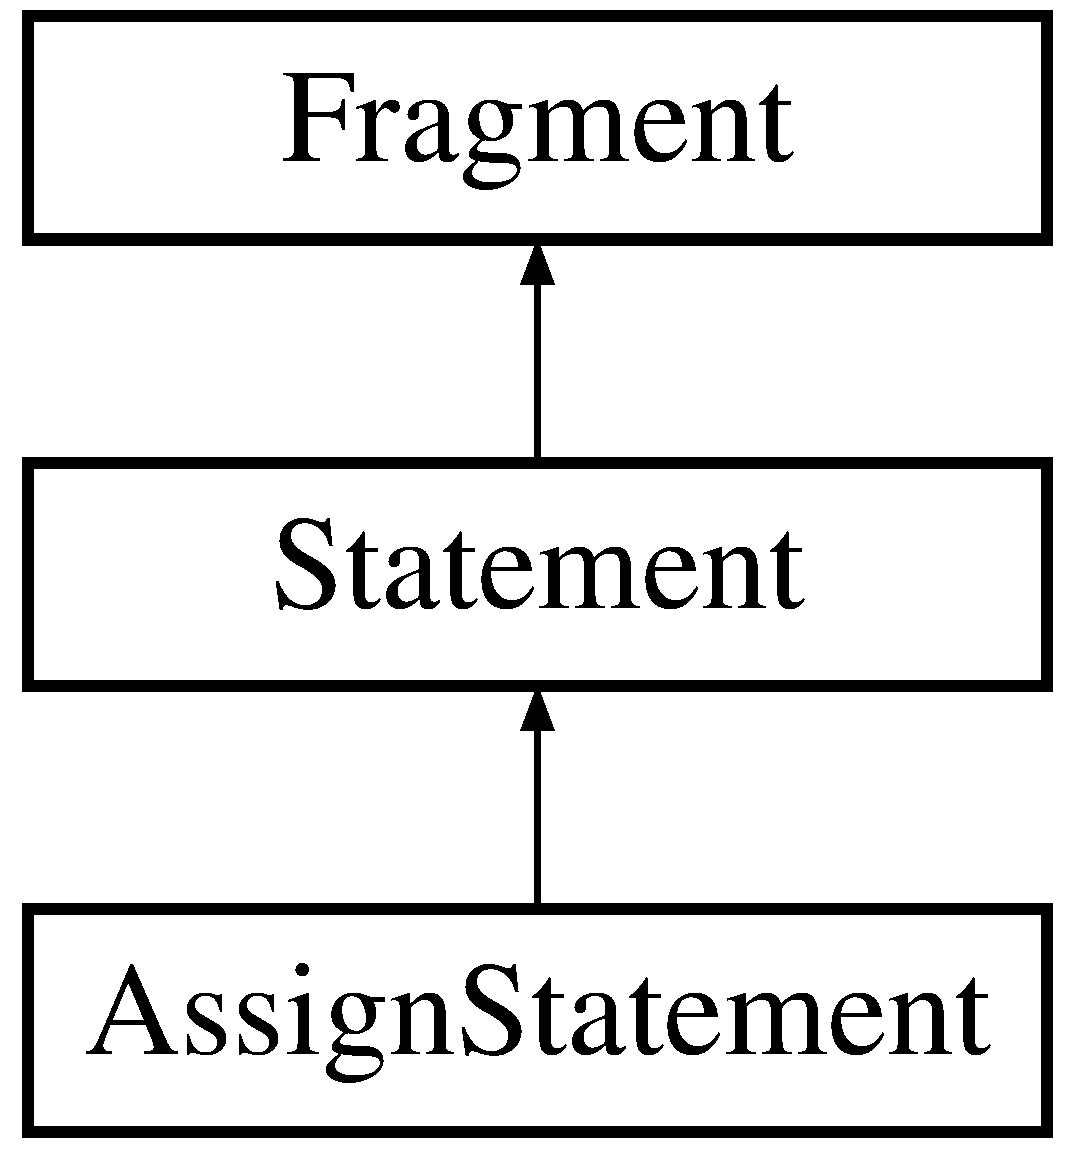
\includegraphics[height=3.000000cm]{d1/d7c/a00003}
\end{center}
\end{figure}
\subsection*{Public Member Functions}
\begin{DoxyCompactItemize}
\item 
\hypertarget{a00003_a6960b0f10c9e5301befe2ab8da9fbd8e}{void {\bfseries parse\+Fragment} (\hyperlink{a00026}{Tokens} $\ast$a\+Tokens, \hyperlink{a00017}{Parser} $\ast$a\+Parser)}\label{a00003_a6960b0f10c9e5301befe2ab8da9fbd8e}

\item 
\hypertarget{a00003_aab1c8b0b2f087014fc096474bc2854ab}{void {\bfseries provide\+Intermediates} (\hyperlink{a00015}{Operation\+Code} $\ast$a\+Opcode, \hyperlink{a00017}{Parser} $\ast$a\+Parser)}\label{a00003_aab1c8b0b2f087014fc096474bc2854ab}

\end{DoxyCompactItemize}
\subsection*{Additional Inherited Members}


The documentation for this class was generated from the following files\+:\begin{DoxyCompactItemize}
\item 
E\+:/\+Projects/backup dropbox/\+Scripting/\+Aiki/\+Compiler/Statement.\+hpp\item 
E\+:/\+Projects/backup dropbox/\+Scripting/\+Aiki/\+Compiler/Statement.\+cpp\end{DoxyCompactItemize}

\hypertarget{a00004}{\section{Byte\+Operation Class Reference}
\label{a00004}\index{Byte\+Operation@{Byte\+Operation}}
}
Inheritance diagram for Byte\+Operation\+:\begin{figure}[H]
\begin{center}
\leavevmode
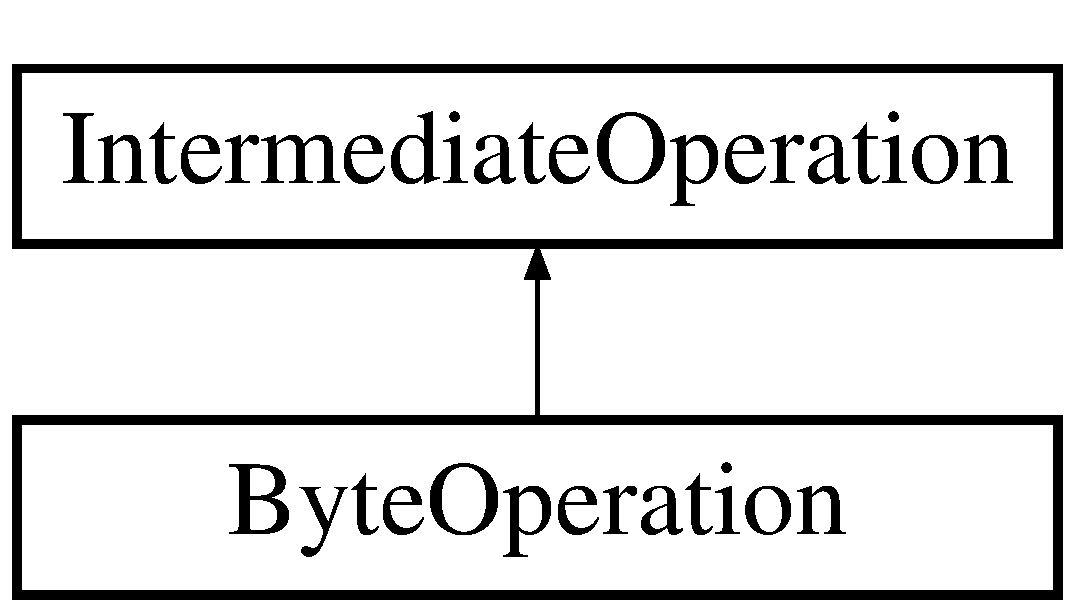
\includegraphics[height=2.000000cm]{d0/d0b/a00004}
\end{center}
\end{figure}
\subsection*{Public Member Functions}
\begin{DoxyCompactItemize}
\item 
\hypertarget{a00004_a543d45bb590172595c94e311316b8867}{{\bfseries Byte\+Operation} (byte a\+Val)}\label{a00004_a543d45bb590172595c94e311316b8867}

\item 
\hypertarget{a00004_a800ac43c60473150dfe5065a0d11156f}{virtual void {\bfseries provide\+Bytecode} (\hyperlink{a00015}{Operation\+Code} $\ast$a\+Opcode)}\label{a00004_a800ac43c60473150dfe5065a0d11156f}

\end{DoxyCompactItemize}
\subsection*{Protected Attributes}
\begin{DoxyCompactItemize}
\item 
\hypertarget{a00004_a8d178848a7de61060bb4ff11c8d7b816}{byte {\bfseries bytes}}\label{a00004_a8d178848a7de61060bb4ff11c8d7b816}

\end{DoxyCompactItemize}


The documentation for this class was generated from the following files\+:\begin{DoxyCompactItemize}
\item 
E\+:/\+Projects/backup dropbox/\+Scripting/\+Aiki/\+Compiler/Intermediate\+Oper.\+hpp\item 
E\+:/\+Projects/backup dropbox/\+Scripting/\+Aiki/\+Compiler/Intermediate\+Oper.\+cpp\end{DoxyCompactItemize}

\hypertarget{a00005}{\section{Dword\+Operation Class Reference}
\label{a00005}\index{Dword\+Operation@{Dword\+Operation}}
}
Inheritance diagram for Dword\+Operation\+:\begin{figure}[H]
\begin{center}
\leavevmode
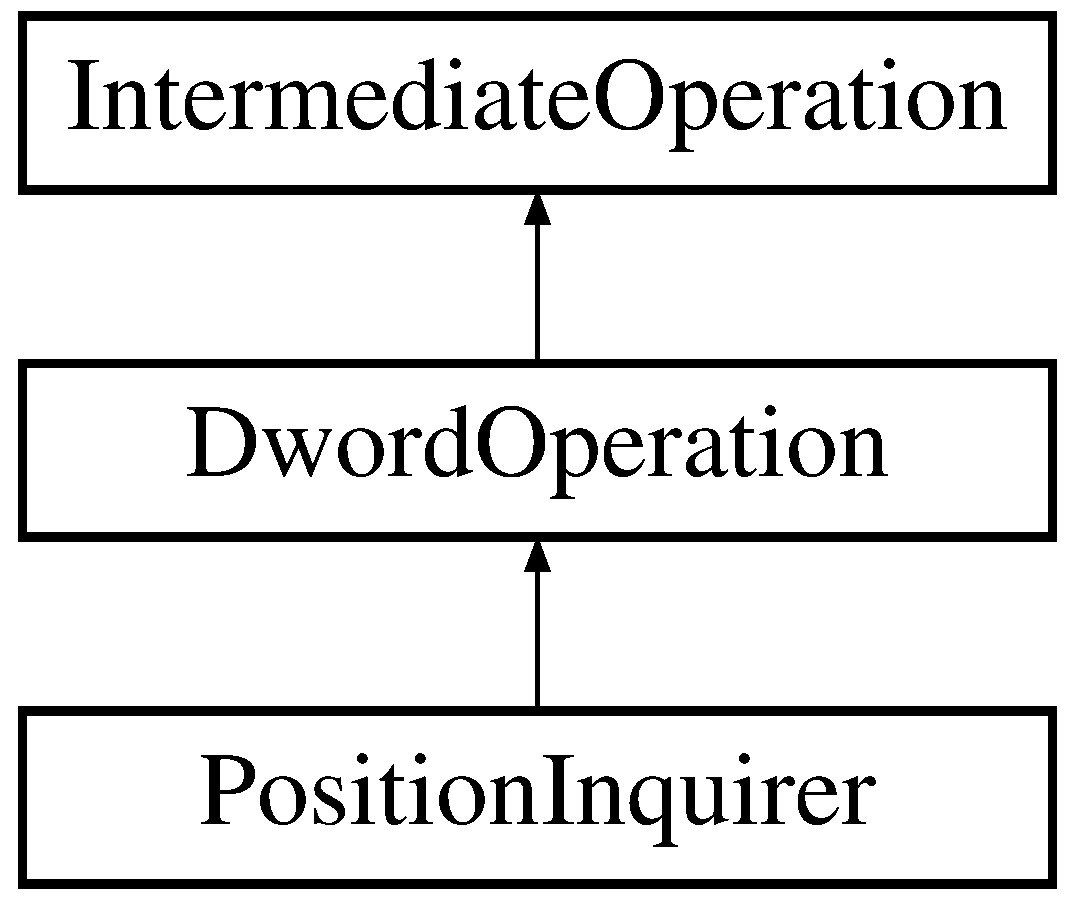
\includegraphics[height=3.000000cm]{dd/dad/a00005}
\end{center}
\end{figure}
\subsection*{Public Member Functions}
\begin{DoxyCompactItemize}
\item 
\hypertarget{a00005_a5dd015cd5a7d49768cfa1fcb70e0fe91}{{\bfseries Dword\+Operation} (void $\ast$a\+Dword)}\label{a00005_a5dd015cd5a7d49768cfa1fcb70e0fe91}

\item 
\hypertarget{a00005_abd70e7feb092ceb2c28c836addfb4ba4}{virtual void {\bfseries provide\+Bytecode} (\hyperlink{a00015}{Operation\+Code} $\ast$a\+Opcode)}\label{a00005_abd70e7feb092ceb2c28c836addfb4ba4}

\end{DoxyCompactItemize}
\subsection*{Protected Attributes}
\begin{DoxyCompactItemize}
\item 
\hypertarget{a00005_a78898cf72cefdba90a87b6ec9b1d1708}{void $\ast$ {\bfseries dword}}\label{a00005_a78898cf72cefdba90a87b6ec9b1d1708}

\end{DoxyCompactItemize}


The documentation for this class was generated from the following files\+:\begin{DoxyCompactItemize}
\item 
E\+:/\+Projects/backup dropbox/\+Scripting/\+Aiki/\+Compiler/Intermediate\+Oper.\+hpp\item 
E\+:/\+Projects/backup dropbox/\+Scripting/\+Aiki/\+Compiler/Intermediate\+Oper.\+cpp\end{DoxyCompactItemize}

\hypertarget{a00006}{\section{Environment Class Reference}
\label{a00006}\index{Environment@{Environment}}
}
\subsection*{Public Member Functions}
\begin{DoxyCompactItemize}
\item 
\hypertarget{a00006_a48378b6044373edbcf5ed4dfd9f53b53}{{\bfseries Environment} (\hyperlink{a00015}{Operation\+Code} $\ast$a\+Opcode)}\label{a00006_a48378b6044373edbcf5ed4dfd9f53b53}

\item 
\hypertarget{a00006_a6b4bdfcd11e23fdd24efab9d33b8734d}{int {\bfseries Execute} ()}\label{a00006_a6b4bdfcd11e23fdd24efab9d33b8734d}

\end{DoxyCompactItemize}


The documentation for this class was generated from the following files\+:\begin{DoxyCompactItemize}
\item 
E\+:/\+Projects/backup dropbox/\+Scripting/\+Aiki/\+Parser/Environment.\+hpp\item 
E\+:/\+Projects/backup dropbox/\+Scripting/\+Aiki/\+Parser/Environment.\+cpp\end{DoxyCompactItemize}

\hypertarget{a00007}{\section{Expression Class Reference}
\label{a00007}\index{Expression@{Expression}}
}
Inheritance diagram for Expression\+:\begin{figure}[H]
\begin{center}
\leavevmode
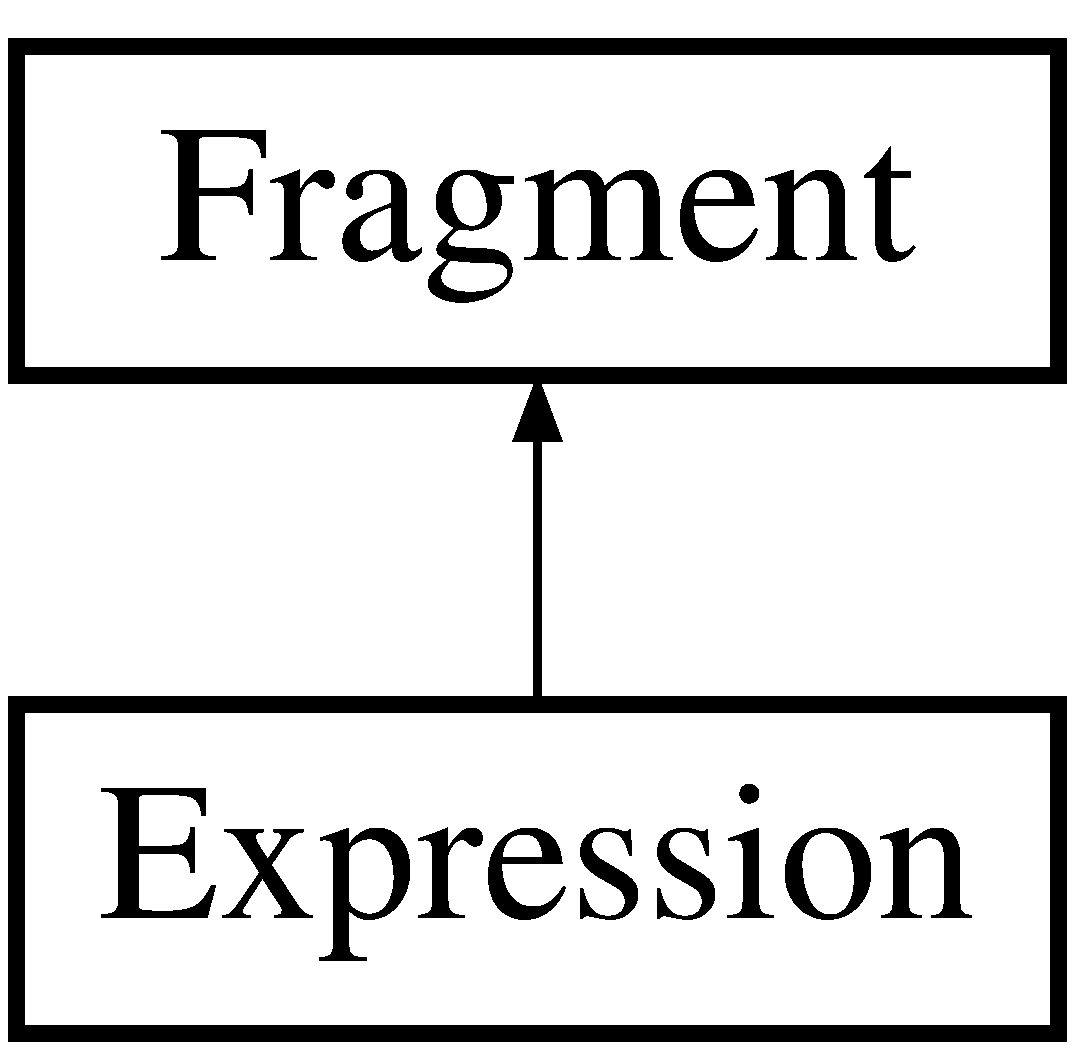
\includegraphics[height=2.000000cm]{de/d5e/a00007}
\end{center}
\end{figure}
\subsection*{Public Member Functions}
\begin{DoxyCompactItemize}
\item 
\hypertarget{a00007_ae3a029c39533808a1c57335628fceed2}{{\bfseries Expression} (bool is\+Function\+Param=false, bool can\+Be\+Null=true)}\label{a00007_ae3a029c39533808a1c57335628fceed2}

\item 
\hypertarget{a00007_a2aad347a1cf9634df14a6bbf8455eb2f}{std\+::string {\bfseries getting\+String} ()}\label{a00007_a2aad347a1cf9634df14a6bbf8455eb2f}

\item 
\hypertarget{a00007_aba5197ed15bc64f8b8d2cb5bca80a96f}{void {\bfseries parse\+Fragment} (\hyperlink{a00026}{Tokens} $\ast$a\+Tokens, \hyperlink{a00017}{Parser} $\ast$a\+Parser)}\label{a00007_aba5197ed15bc64f8b8d2cb5bca80a96f}

\item 
\hypertarget{a00007_a2c210728bcca2511ce480daab2e4842b}{void {\bfseries provide\+Intermediates} (\hyperlink{a00015}{Operation\+Code} $\ast$a\+Opcode, \hyperlink{a00017}{Parser} $\ast$a\+Parser)}\label{a00007_a2c210728bcca2511ce480daab2e4842b}

\end{DoxyCompactItemize}
\subsection*{Additional Inherited Members}


The documentation for this class was generated from the following files\+:\begin{DoxyCompactItemize}
\item 
E\+:/\+Projects/backup dropbox/\+Scripting/\+Aiki/\+Compiler/Expression.\+hpp\item 
E\+:/\+Projects/backup dropbox/\+Scripting/\+Aiki/\+Compiler/Expression.\+cpp\end{DoxyCompactItemize}

\hypertarget{a00008}{\section{Fragment Class Reference}
\label{a00008}\index{Fragment@{Fragment}}
}
Inheritance diagram for Fragment\+:\begin{figure}[H]
\begin{center}
\leavevmode
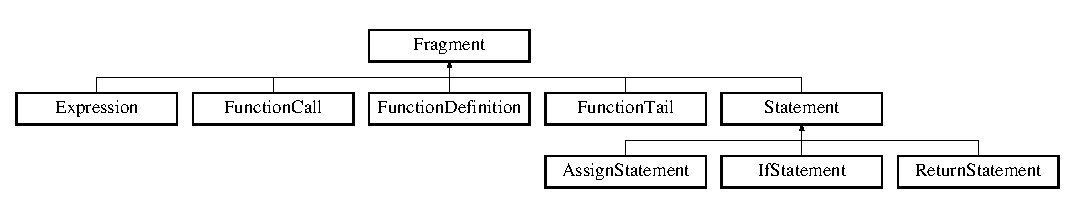
\includegraphics[height=2.295082cm]{d4/dee/a00008}
\end{center}
\end{figure}
\subsection*{Public Member Functions}
\begin{DoxyCompactItemize}
\item 
\hypertarget{a00008_a1d02e878454a0146177d80c8a8ef4b8c}{virtual void {\bfseries parse\+Fragment} (\hyperlink{a00026}{Tokens} $\ast$a\+Tokens, \hyperlink{a00017}{Parser} $\ast$a\+Parser)=0}\label{a00008_a1d02e878454a0146177d80c8a8ef4b8c}

\item 
\hypertarget{a00008_a2b367d190ab530604d1d7019d1e60612}{virtual void {\bfseries provide\+Intermediates} (\hyperlink{a00015}{Operation\+Code} $\ast$a\+Opcode, \hyperlink{a00017}{Parser} $\ast$a\+Parser)=0}\label{a00008_a2b367d190ab530604d1d7019d1e60612}

\item 
\hypertarget{a00008_a144b839eeb8c9f4dcd3ccacb81db8417}{virtual std\+::string {\bfseries getting\+String} ()}\label{a00008_a144b839eeb8c9f4dcd3ccacb81db8417}

\end{DoxyCompactItemize}
\subsection*{Protected Member Functions}
\begin{DoxyCompactItemize}
\item 
\hypertarget{a00008_ab11b535d467a5e46665f6536240eb9cc}{uint {\bfseries set\+Variable} (\hyperlink{a00017}{Parser} $\ast$a\+Parser, std\+::string a\+Name)}\label{a00008_ab11b535d467a5e46665f6536240eb9cc}

\item 
\hypertarget{a00008_a01e2bbf3887a4ade067110d1832740e4}{uint {\bfseries get\+Variable\+I\+D} (\hyperlink{a00017}{Parser} $\ast$a\+Parser, std\+::string a\+Name)}\label{a00008_a01e2bbf3887a4ade067110d1832740e4}

\item 
\hypertarget{a00008_a1fc143f43ea9a57d08a2f144bc190572}{void {\bfseries allocate\+Variable} (\hyperlink{a00015}{Operation\+Code} $\ast$a\+Operation\+Code, uint a\+Variable\+I\+D)}\label{a00008_a1fc143f43ea9a57d08a2f144bc190572}

\end{DoxyCompactItemize}


The documentation for this class was generated from the following files\+:\begin{DoxyCompactItemize}
\item 
E\+:/\+Projects/backup dropbox/\+Scripting/\+Aiki/\+Compiler/Fragment.\+hpp\item 
E\+:/\+Projects/backup dropbox/\+Scripting/\+Aiki/\+Compiler/Fragment.\+cpp\end{DoxyCompactItemize}

\hypertarget{a00009}{\section{Function\+Call Class Reference}
\label{a00009}\index{Function\+Call@{Function\+Call}}
}
Inheritance diagram for Function\+Call\+:\begin{figure}[H]
\begin{center}
\leavevmode
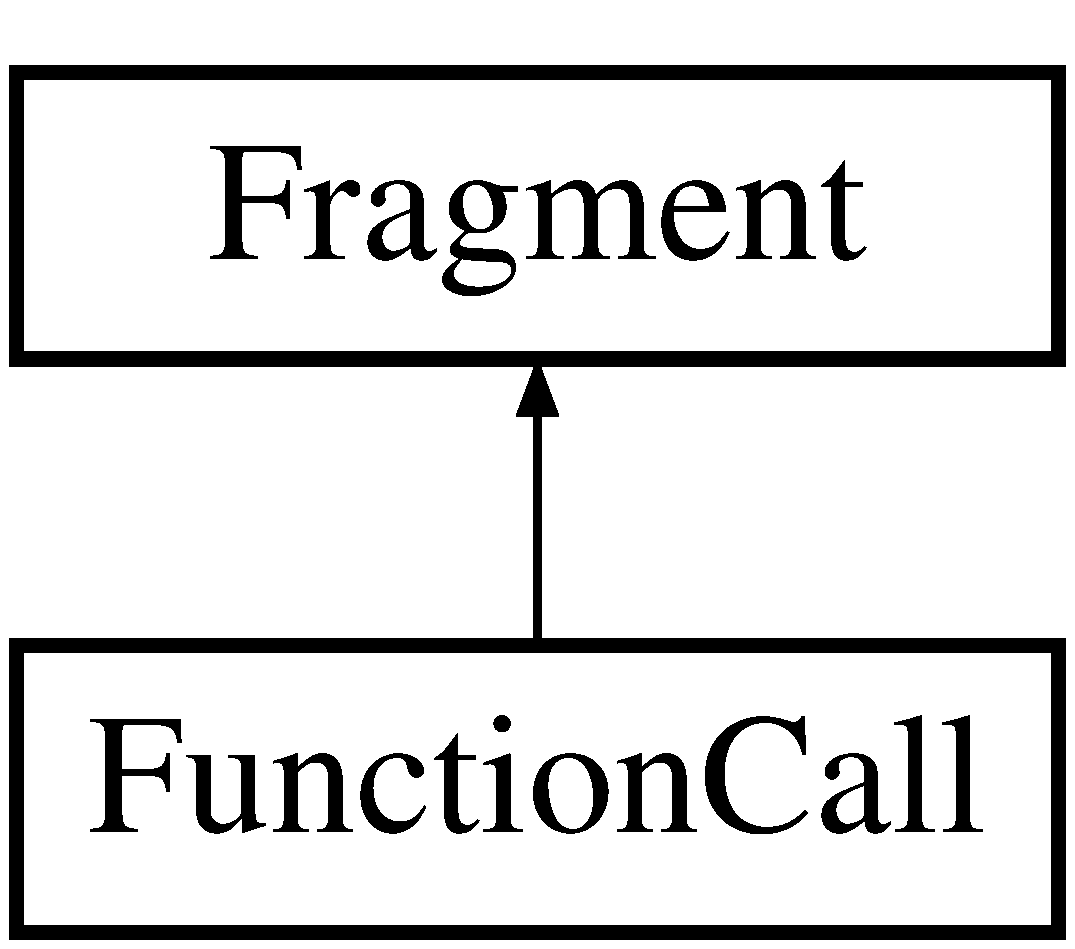
\includegraphics[height=2.000000cm]{da/da0/a00009}
\end{center}
\end{figure}
\subsection*{Public Member Functions}
\begin{DoxyCompactItemize}
\item 
\hypertarget{a00009_a6fc104abe67e06bc350b382078154016}{{\bfseries Function\+Call} (\hyperlink{a00025}{Token} $\ast$a\+Func\+Token)}\label{a00009_a6fc104abe67e06bc350b382078154016}

\item 
\hypertarget{a00009_ae9e672734e8d1256da3c47982d43aa82}{void {\bfseries parse\+Fragment} (\hyperlink{a00026}{Tokens} $\ast$a\+Tokens, \hyperlink{a00017}{Parser} $\ast$a\+Parser)}\label{a00009_ae9e672734e8d1256da3c47982d43aa82}

\item 
\hypertarget{a00009_aeb0aeff829ba6808d93ea8bc51c8de66}{void {\bfseries provide\+Intermediates} (\hyperlink{a00015}{Operation\+Code} $\ast$a\+Opcode, \hyperlink{a00017}{Parser} $\ast$a\+Parser)}\label{a00009_aeb0aeff829ba6808d93ea8bc51c8de66}

\item 
\hypertarget{a00009_a0e9cb53ae74b3a0c096f590d8a46ec6d}{std\+::string {\bfseries get\+String} ()}\label{a00009_a0e9cb53ae74b3a0c096f590d8a46ec6d}

\end{DoxyCompactItemize}
\subsection*{Protected Member Functions}
\begin{DoxyCompactItemize}
\item 
\hypertarget{a00009_ad46b2bedbc4e32b902639f02e8b980d4}{void {\bfseries handle\+Parameters} (\hyperlink{a00015}{Operation\+Code} $\ast$a\+Opcode, \hyperlink{a00017}{Parser} $\ast$a\+Parser)}\label{a00009_ad46b2bedbc4e32b902639f02e8b980d4}

\end{DoxyCompactItemize}
\subsection*{Protected Attributes}
\begin{DoxyCompactItemize}
\item 
\hypertarget{a00009_aaa4480d7bf30a98289bf80d7aeff4430}{Token\+::\+Type {\bfseries delimter}}\label{a00009_aaa4480d7bf30a98289bf80d7aeff4430}

\item 
\hypertarget{a00009_aeeb16256fafa10242b270d4bf417bad0}{\hyperlink{a00025}{Token} $\ast$ {\bfseries function\+Token}}\label{a00009_aeeb16256fafa10242b270d4bf417bad0}

\item 
\hypertarget{a00009_a43942cc2f7ea191f6d3104d5bbac1e83}{std\+::list$<$ \hyperlink{a00007}{Expression} $\ast$ $>$ {\bfseries parameters}}\label{a00009_a43942cc2f7ea191f6d3104d5bbac1e83}

\end{DoxyCompactItemize}


The documentation for this class was generated from the following files\+:\begin{DoxyCompactItemize}
\item 
E\+:/\+Projects/backup dropbox/\+Scripting/\+Aiki/\+Compiler/Function.\+hpp\item 
E\+:/\+Projects/backup dropbox/\+Scripting/\+Aiki/\+Compiler/Function.\+cpp\end{DoxyCompactItemize}

\hypertarget{a00010}{\section{Function\+Definition Class Reference}
\label{a00010}\index{Function\+Definition@{Function\+Definition}}
}
Inheritance diagram for Function\+Definition\+:\begin{figure}[H]
\begin{center}
\leavevmode
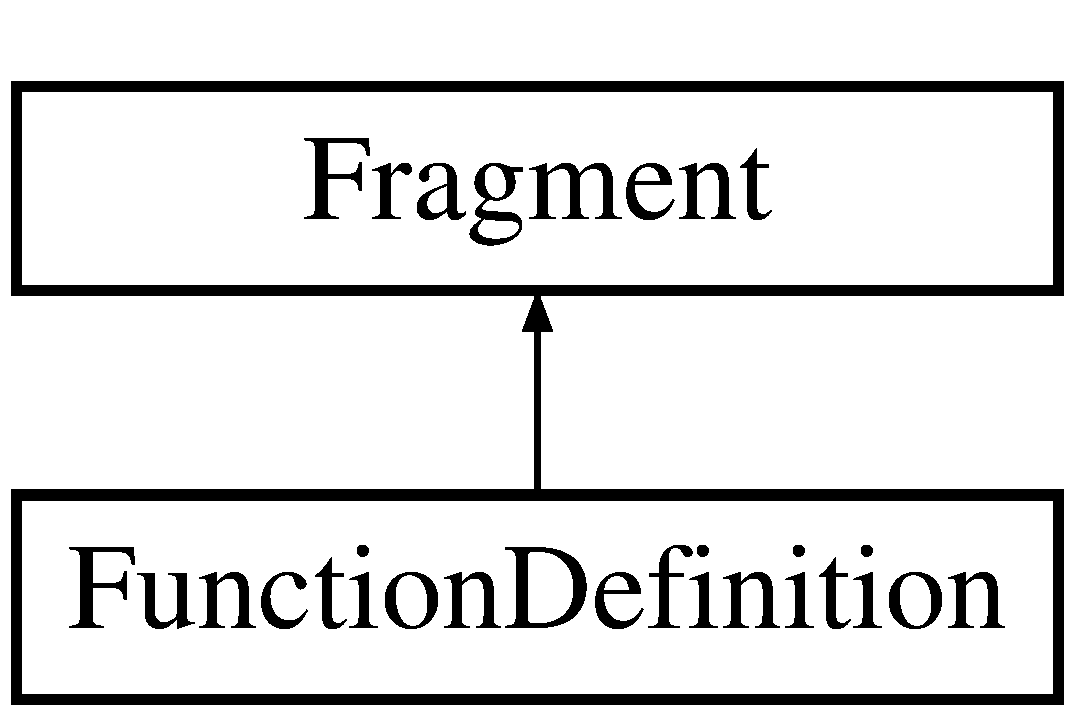
\includegraphics[height=2.000000cm]{d7/dec/a00010}
\end{center}
\end{figure}
\subsection*{Public Member Functions}
\begin{DoxyCompactItemize}
\item 
\hypertarget{a00010_a58c9debf23ec862b0d920d7f3231e2a2}{\hyperlink{a00019}{Position\+Reference} $\ast$ {\bfseries get\+Position\+Reference} ()}\label{a00010_a58c9debf23ec862b0d920d7f3231e2a2}

\item 
\hypertarget{a00010_af6129d50e3f39cb8b318f68a235df94a}{void {\bfseries parse\+Fragment} (\hyperlink{a00026}{Tokens} $\ast$a\+Tokens, \hyperlink{a00017}{Parser} $\ast$a\+Parser)}\label{a00010_af6129d50e3f39cb8b318f68a235df94a}

\item 
\hypertarget{a00010_ad71d600ad87b03c4d6d1d4c906e91795}{void {\bfseries provide\+Intermediates} (\hyperlink{a00015}{Operation\+Code} $\ast$a\+Opcode, \hyperlink{a00017}{Parser} $\ast$a\+Parser)}\label{a00010_ad71d600ad87b03c4d6d1d4c906e91795}

\item 
\hypertarget{a00010_a111684d7a2147f1541e88d9ec2692a39}{uint {\bfseries get\+I\+D} ()}\label{a00010_a111684d7a2147f1541e88d9ec2692a39}

\end{DoxyCompactItemize}
\subsection*{Static Public Member Functions}
\begin{DoxyCompactItemize}
\item 
\hypertarget{a00010_aa5559af30e7e7e4aa3be29be6b3bda7e}{static bool {\bfseries is\+Function\+Definition} (\hyperlink{a00026}{Tokens} $\ast$a\+Tokens)}\label{a00010_aa5559af30e7e7e4aa3be29be6b3bda7e}

\end{DoxyCompactItemize}
\subsection*{Protected Attributes}
\begin{DoxyCompactItemize}
\item 
\hypertarget{a00010_a60ebd403b26d523eff61d2a64fb27844}{std\+::list$<$ \hyperlink{a00025}{Token} $\ast$ $>$ {\bfseries parameter}}\label{a00010_a60ebd403b26d523eff61d2a64fb27844}

\item 
\hypertarget{a00010_a47075e621f8a25d995dc9cf8a0a116fe}{\hyperlink{a00019}{Position\+Reference} $\ast$ {\bfseries position\+Reference}}\label{a00010_a47075e621f8a25d995dc9cf8a0a116fe}

\item 
\hypertarget{a00010_a575ea1e569ce84b127ca0a7a8e0a6d00}{uint {\bfseries function\+I\+D}}\label{a00010_a575ea1e569ce84b127ca0a7a8e0a6d00}

\end{DoxyCompactItemize}
\subsection*{Additional Inherited Members}


The documentation for this class was generated from the following files\+:\begin{DoxyCompactItemize}
\item 
E\+:/\+Projects/backup dropbox/\+Scripting/\+Aiki/\+Compiler/Function.\+hpp\item 
E\+:/\+Projects/backup dropbox/\+Scripting/\+Aiki/\+Compiler/Function.\+cpp\end{DoxyCompactItemize}

\hypertarget{a00011}{\section{Function\+Signature Class Reference}
\label{a00011}\index{Function\+Signature@{Function\+Signature}}
}
\subsection*{Public Member Functions}
\begin{DoxyCompactItemize}
\item 
\hypertarget{a00011_a2b563532d18fb61145c005ca5ce9c460}{{\bfseries Function\+Signature} (std\+::string a\+Name, int a\+Params)}\label{a00011_a2b563532d18fb61145c005ca5ce9c460}

\item 
\hypertarget{a00011_a785ace56c6b09896a075e282dccc3b53}{std\+::string {\bfseries get\+Name} ()}\label{a00011_a785ace56c6b09896a075e282dccc3b53}

\item 
\hypertarget{a00011_ade2d65b7212c39caa2ad5a48550f464d}{int {\bfseries get\+Parameter\+Count} ()}\label{a00011_ade2d65b7212c39caa2ad5a48550f464d}

\item 
\hypertarget{a00011_a4b86cb0d46a2c03fe32714c4313e58d2}{uint {\bfseries get\+I\+D} ()}\label{a00011_a4b86cb0d46a2c03fe32714c4313e58d2}

\item 
\hypertarget{a00011_a882b70c9d2e096f355ccca91962cc9e2}{void {\bfseries set\+I\+D} (uint a\+I\+D)}\label{a00011_a882b70c9d2e096f355ccca91962cc9e2}

\end{DoxyCompactItemize}


The documentation for this class was generated from the following files\+:\begin{DoxyCompactItemize}
\item 
E\+:/\+Projects/backup dropbox/\+Scripting/\+Aiki/\+Compiler/Function.\+hpp\item 
E\+:/\+Projects/backup dropbox/\+Scripting/\+Aiki/\+Compiler/Function.\+cpp\end{DoxyCompactItemize}

\hypertarget{a00012}{\section{Function\+Tail Class Reference}
\label{a00012}\index{Function\+Tail@{Function\+Tail}}
}
Inheritance diagram for Function\+Tail\+:\begin{figure}[H]
\begin{center}
\leavevmode
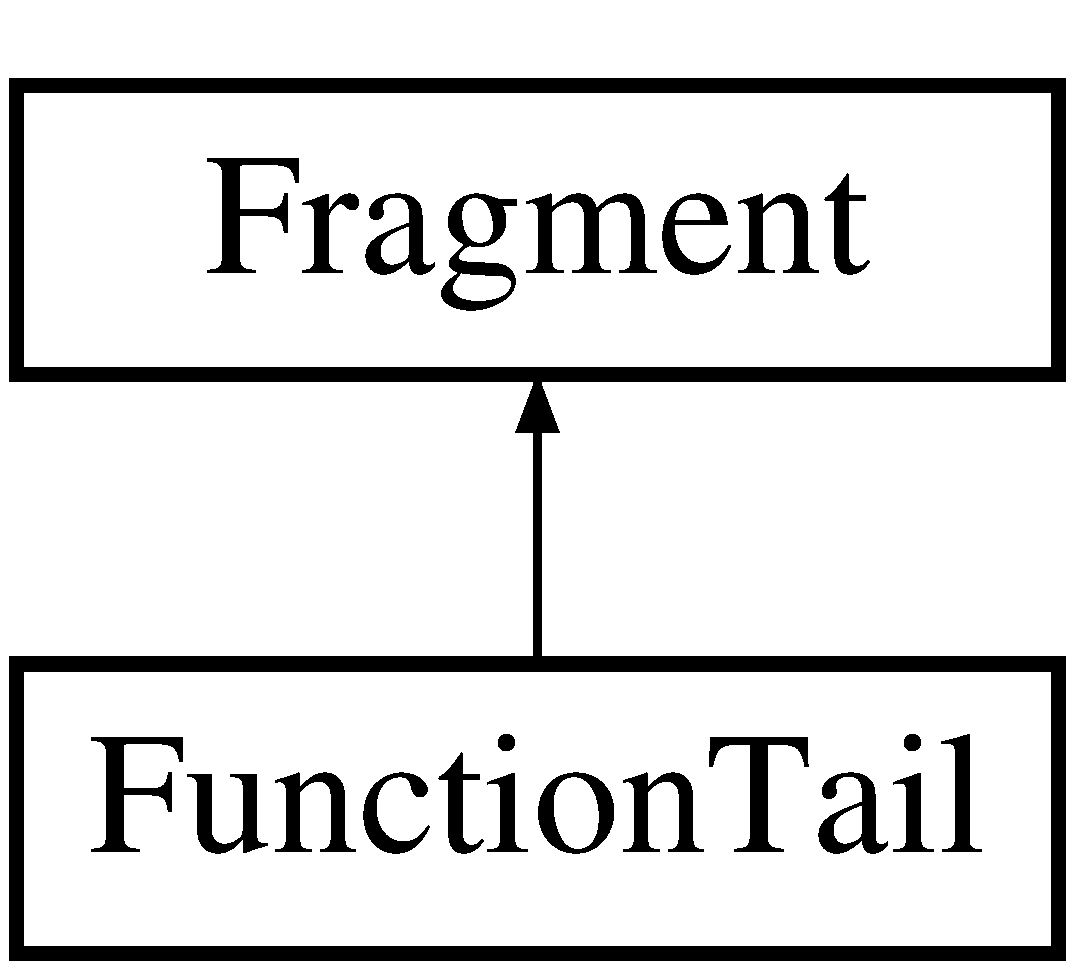
\includegraphics[height=2.000000cm]{df/d86/a00012}
\end{center}
\end{figure}
\subsection*{Public Member Functions}
\begin{DoxyCompactItemize}
\item 
\hypertarget{a00012_a903ff1fe2254630df3fa6b13424a32da}{void {\bfseries parse\+Fragment} (\hyperlink{a00026}{Tokens} $\ast$a\+Tokens, \hyperlink{a00017}{Parser} $\ast$a\+Parser)}\label{a00012_a903ff1fe2254630df3fa6b13424a32da}

\item 
\hypertarget{a00012_a1d05757a48e27d1cb8cca922f7303044}{void {\bfseries provide\+Intermediates} (\hyperlink{a00015}{Operation\+Code} $\ast$a\+Opcode, \hyperlink{a00017}{Parser} $\ast$a\+Parser)}\label{a00012_a1d05757a48e27d1cb8cca922f7303044}

\item 
\hypertarget{a00012_af930cde44d6b891ff83abc154d246e95}{\hyperlink{a00019}{Position\+Reference} $\ast$ {\bfseries get\+Position\+Reference} ()}\label{a00012_af930cde44d6b891ff83abc154d246e95}

\end{DoxyCompactItemize}
\subsection*{Additional Inherited Members}


The documentation for this class was generated from the following files\+:\begin{DoxyCompactItemize}
\item 
E\+:/\+Projects/backup dropbox/\+Scripting/\+Aiki/\+Compiler/Function.\+hpp\item 
E\+:/\+Projects/backup dropbox/\+Scripting/\+Aiki/\+Compiler/Function.\+cpp\end{DoxyCompactItemize}

\hypertarget{a00013}{\section{If\+Statement Class Reference}
\label{a00013}\index{If\+Statement@{If\+Statement}}
}
Inheritance diagram for If\+Statement\+:\begin{figure}[H]
\begin{center}
\leavevmode
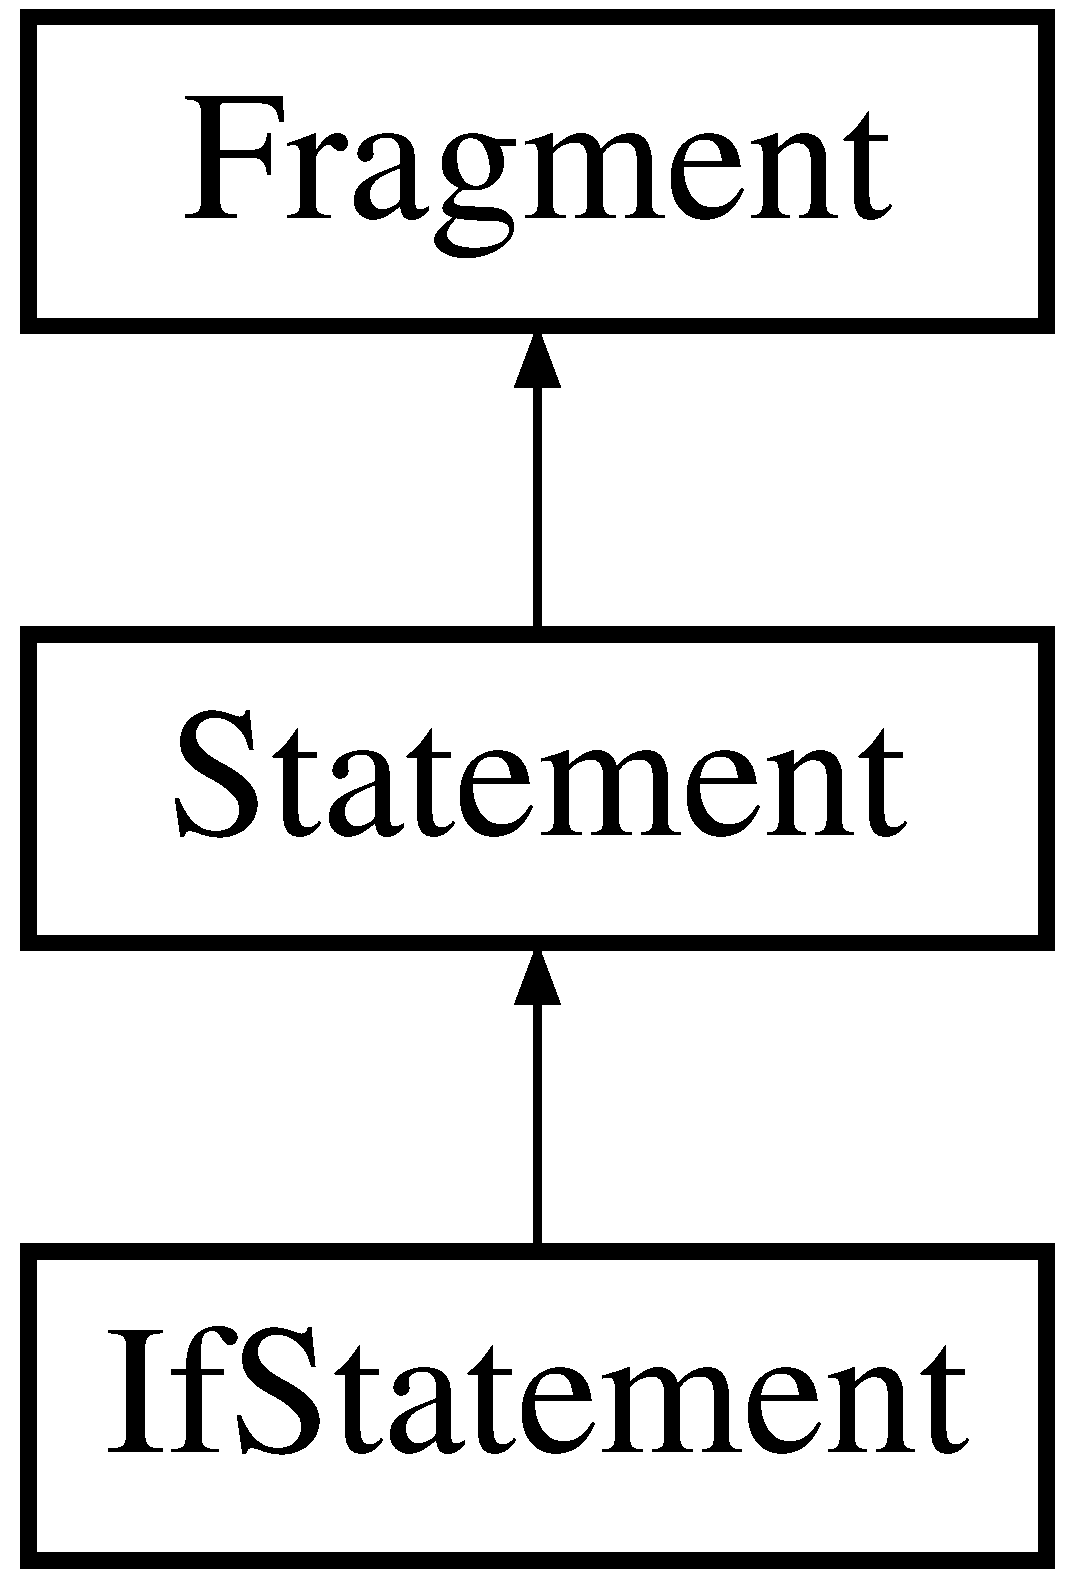
\includegraphics[height=3.000000cm]{d7/dd4/a00013}
\end{center}
\end{figure}
\subsection*{Public Member Functions}
\begin{DoxyCompactItemize}
\item 
\hypertarget{a00013_a2dcef21fb3f3d969007df235e01f6900}{void {\bfseries parse\+Fragment} (\hyperlink{a00026}{Tokens} $\ast$a\+Tokens, \hyperlink{a00017}{Parser} $\ast$a\+Parser)}\label{a00013_a2dcef21fb3f3d969007df235e01f6900}

\item 
\hypertarget{a00013_a90f085925b7ef5edce272f3294d8c047}{void {\bfseries provide\+Intermediates} (\hyperlink{a00015}{Operation\+Code} $\ast$a\+Opcode, \hyperlink{a00017}{Parser} $\ast$a\+Parser)}\label{a00013_a90f085925b7ef5edce272f3294d8c047}

\end{DoxyCompactItemize}
\subsection*{Additional Inherited Members}


The documentation for this class was generated from the following files\+:\begin{DoxyCompactItemize}
\item 
E\+:/\+Projects/backup dropbox/\+Scripting/\+Aiki/\+Compiler/Statement.\+hpp\item 
E\+:/\+Projects/backup dropbox/\+Scripting/\+Aiki/\+Compiler/Statement.\+cpp\end{DoxyCompactItemize}

\hypertarget{a00014}{\section{Intermediate\+Operation Class Reference}
\label{a00014}\index{Intermediate\+Operation@{Intermediate\+Operation}}
}
Inheritance diagram for Intermediate\+Operation\+:\begin{figure}[H]
\begin{center}
\leavevmode
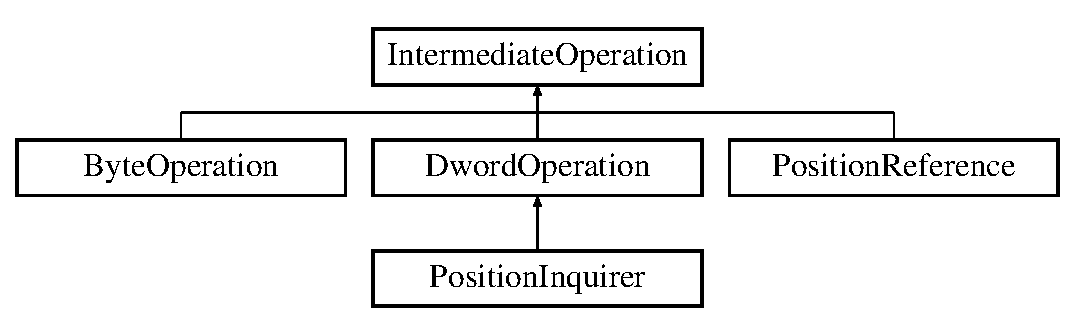
\includegraphics[height=3.000000cm]{d2/de7/a00014}
\end{center}
\end{figure}
\subsection*{Public Member Functions}
\begin{DoxyCompactItemize}
\item 
\hypertarget{a00014_aefbe33217f1ab8d3b4338beb11ed9911}{virtual void {\bfseries provide\+Bytecode} (\hyperlink{a00015}{Operation\+Code} $\ast$a\+Opcode)=0}\label{a00014_aefbe33217f1ab8d3b4338beb11ed9911}

\end{DoxyCompactItemize}


The documentation for this class was generated from the following file\+:\begin{DoxyCompactItemize}
\item 
E\+:/\+Projects/backup dropbox/\+Scripting/\+Aiki/\+Compiler/Intermediate\+Oper.\+hpp\end{DoxyCompactItemize}

\hypertarget{a00015}{\section{Operation\+Code Class Reference}
\label{a00015}\index{Operation\+Code@{Operation\+Code}}
}
\subsection*{Public Member Functions}
\begin{DoxyCompactItemize}
\item 
\hypertarget{a00015_ac0f1c51ea1fb3dca7c12df8b40a3a9fc}{bool {\bfseries is\+Big\+End} ()}\label{a00015_ac0f1c51ea1fb3dca7c12df8b40a3a9fc}

\item 
\hypertarget{a00015_aea26ab3a3870c339f645fcf08393d7ff}{const vector$<$ byte $>$ {\bfseries get\+Bytecode} ()}\label{a00015_aea26ab3a3870c339f645fcf08393d7ff}

\item 
\hypertarget{a00015_a86ecde320164c35c4bbfde1d84004382}{int {\bfseries length} ()}\label{a00015_a86ecde320164c35c4bbfde1d84004382}

\item 
\hypertarget{a00015_aa677fbb79b000236e51cb58f8914efdd}{Interop\+Iter {\bfseries add\+Interop} (\hyperlink{a00014}{Intermediate\+Operation} $\ast$interop)}\label{a00015_aa677fbb79b000236e51cb58f8914efdd}

\item 
\hypertarget{a00015_af582b3766d98cb4dc03b52715b4245ab}{void {\bfseries push\+Tail} (Interop\+Iter it)}\label{a00015_af582b3766d98cb4dc03b52715b4245ab}

\item 
\hypertarget{a00015_a851082a0d4198802422289c3a9fa6c2e}{void {\bfseries pop\+Tail} ()}\label{a00015_a851082a0d4198802422289c3a9fa6c2e}

\item 
\hypertarget{a00015_ac4933dc30cf05ea38c1ba362d716fbcc}{bool {\bfseries build\+Bytecode\+From\+Intermediates} ()}\label{a00015_ac4933dc30cf05ea38c1ba362d716fbcc}

\item 
\hypertarget{a00015_ad3fd8287bebf2b2ce10268afd294fa0c}{\hyperlink{a00015}{Operation\+Code} $\ast$ {\bfseries add\+Byte} (byte val)}\label{a00015_ad3fd8287bebf2b2ce10268afd294fa0c}

\item 
\hypertarget{a00015_a454dad1134c629f0611f81bf10c62423}{\hyperlink{a00015}{Operation\+Code} $\ast$ {\bfseries add\+Dword} (void $\ast$dword)}\label{a00015_a454dad1134c629f0611f81bf10c62423}

\item 
\hypertarget{a00015_a2eef4417f202cef42b6ff21ae7c13681}{\hyperlink{a00015}{Operation\+Code} $\ast$ {\bfseries add\+Int} (int val)}\label{a00015_a2eef4417f202cef42b6ff21ae7c13681}

\item 
\hypertarget{a00015_a12f4b8427569261595a535d6815d64ce}{\hyperlink{a00015}{Operation\+Code} $\ast$ {\bfseries add\+Uint} (uint val)}\label{a00015_a12f4b8427569261595a535d6815d64ce}

\item 
\hypertarget{a00015_a19153b35fd9800909a27ea787f0e791f}{void {\bfseries replace\+Byte} (int index, byte val)}\label{a00015_a19153b35fd9800909a27ea787f0e791f}

\item 
\hypertarget{a00015_a81ac6d741fefd5decbba3cd6a1f37cc2}{void {\bfseries replace\+Uint} (int index, uint val)}\label{a00015_a81ac6d741fefd5decbba3cd6a1f37cc2}

\end{DoxyCompactItemize}


The documentation for this class was generated from the following files\+:\begin{DoxyCompactItemize}
\item 
E\+:/\+Projects/backup dropbox/\+Scripting/\+Aiki/Operation\+Code.\+hpp\item 
E\+:/\+Projects/backup dropbox/\+Scripting/\+Aiki/Operation\+Code.\+cpp\end{DoxyCompactItemize}

\hypertarget{a00016}{\section{Operation\+Code\+Text Class Reference}
\label{a00016}\index{Operation\+Code\+Text@{Operation\+Code\+Text}}
}
\subsection*{Public Member Functions}
\begin{DoxyCompactItemize}
\item 
\hypertarget{a00016_ac7a997e924fdd8217194b4770cec8190}{void {\bfseries parse} (\hyperlink{a00015}{Operation\+Code} $\ast$a\+Operation\+Code)}\label{a00016_ac7a997e924fdd8217194b4770cec8190}

\end{DoxyCompactItemize}


The documentation for this class was generated from the following files\+:\begin{DoxyCompactItemize}
\item 
E\+:/\+Projects/backup dropbox/\+Scripting/\+Aiki/Operation\+Code\+Text.\+hpp\item 
E\+:/\+Projects/backup dropbox/\+Scripting/\+Aiki/Operation\+Code\+Text.\+cpp\end{DoxyCompactItemize}

\hypertarget{a00017}{\section{Parser Class Reference}
\label{a00017}\index{Parser@{Parser}}
}
\subsection*{Public Member Functions}
\begin{DoxyCompactItemize}
\item 
\hypertarget{a00017_a035c46274311501757564dfbaf052f2d}{{\bfseries Parser} (string a\+File, bool a\+Main\+File)}\label{a00017_a035c46274311501757564dfbaf052f2d}

\item 
\hypertarget{a00017_af06133bfc45c2a15c3742c31c1f226c4}{bool {\bfseries parse\+File} ()}\label{a00017_af06133bfc45c2a15c3742c31c1f226c4}

\item 
\hypertarget{a00017_ae536c7f606706a84ff08ce69cb3b5711}{bool {\bfseries compile\+Tokens} ()}\label{a00017_ae536c7f606706a84ff08ce69cb3b5711}

\item 
\hypertarget{a00017_a31b193c27eae5bb43de8921f94ba2707}{\hyperlink{a00015}{Operation\+Code} $\ast$ {\bfseries get\+Opcodes} ()}\label{a00017_a31b193c27eae5bb43de8921f94ba2707}

\item 
\hypertarget{a00017_aac2d2e20c5477b9520cfacd9088f1bee}{void {\bfseries push\+Scope} ()}\label{a00017_aac2d2e20c5477b9520cfacd9088f1bee}

\item 
\hypertarget{a00017_aa249068b5c9f7deb72915e0c25a3d405}{void {\bfseries pop\+Scope} ()}\label{a00017_aa249068b5c9f7deb72915e0c25a3d405}

\item 
\hypertarget{a00017_a0fec5d464e3f94885418b809ae126238}{bool {\bfseries is\+In\+Local\+Scope} ()}\label{a00017_a0fec5d464e3f94885418b809ae126238}

\item 
\hypertarget{a00017_aafd539cf018fb72657fcf913cc2d9532}{void {\bfseries push\+Nested\+Scope} ()}\label{a00017_aafd539cf018fb72657fcf913cc2d9532}

\item 
\hypertarget{a00017_ace4796e2e5308d3190734359cfb1ae54}{void {\bfseries pop\+Nested\+Scope} ()}\label{a00017_ace4796e2e5308d3190734359cfb1ae54}

\item 
\hypertarget{a00017_aace63234361457418d693085582af97c}{uint {\bfseries register\+Variable} (string a\+Name)}\label{a00017_aace63234361457418d693085582af97c}

\item 
\hypertarget{a00017_a24eef3cc93d434d84bf2b3de40745451}{uint {\bfseries get\+Variable\+I\+D} (string a\+Name)}\label{a00017_a24eef3cc93d434d84bf2b3de40745451}

\item 
\hypertarget{a00017_a92f74b87626da42f567a72ed100b4e96}{uint {\bfseries register\+Function} (\hyperlink{a00011}{Function\+Signature} a\+Func\+Sign)}\label{a00017_a92f74b87626da42f567a72ed100b4e96}

\item 
\hypertarget{a00017_a4a53a3a771671d563f221146db903c59}{uint {\bfseries register\+Std\+Function} (\hyperlink{a00011}{Function\+Signature} a\+Func\+Sign)}\label{a00017_a4a53a3a771671d563f221146db903c59}

\item 
\hypertarget{a00017_af8654197b3599c037c1a3f455f4ac819}{uint {\bfseries get\+Function\+I\+D} (string a\+Name)}\label{a00017_af8654197b3599c037c1a3f455f4ac819}

\item 
\hypertarget{a00017_aba4f206134629463121fcd61c40644f2}{\hyperlink{a00011}{Function\+Signature} {\bfseries get\+Function\+Signature} (string a\+Function\+Name)}\label{a00017_aba4f206134629463121fcd61c40644f2}

\item 
\hypertarget{a00017_a1b51b4ba165d214d50ba725428976175}{\hyperlink{a00011}{Function\+Signature} {\bfseries get\+Function\+Signature} (uint a\+Function\+I\+D)}\label{a00017_a1b51b4ba165d214d50ba725428976175}

\end{DoxyCompactItemize}


The documentation for this class was generated from the following files\+:\begin{DoxyCompactItemize}
\item 
E\+:/\+Projects/backup dropbox/\+Scripting/\+Aiki/\+Compiler/Parser.\+hpp\item 
E\+:/\+Projects/backup dropbox/\+Scripting/\+Aiki/\+Compiler/Parser.\+cpp\end{DoxyCompactItemize}

\hypertarget{a00018}{\section{Position\+Inquirer Class Reference}
\label{a00018}\index{Position\+Inquirer@{Position\+Inquirer}}
}
Inheritance diagram for Position\+Inquirer\+:\begin{figure}[H]
\begin{center}
\leavevmode
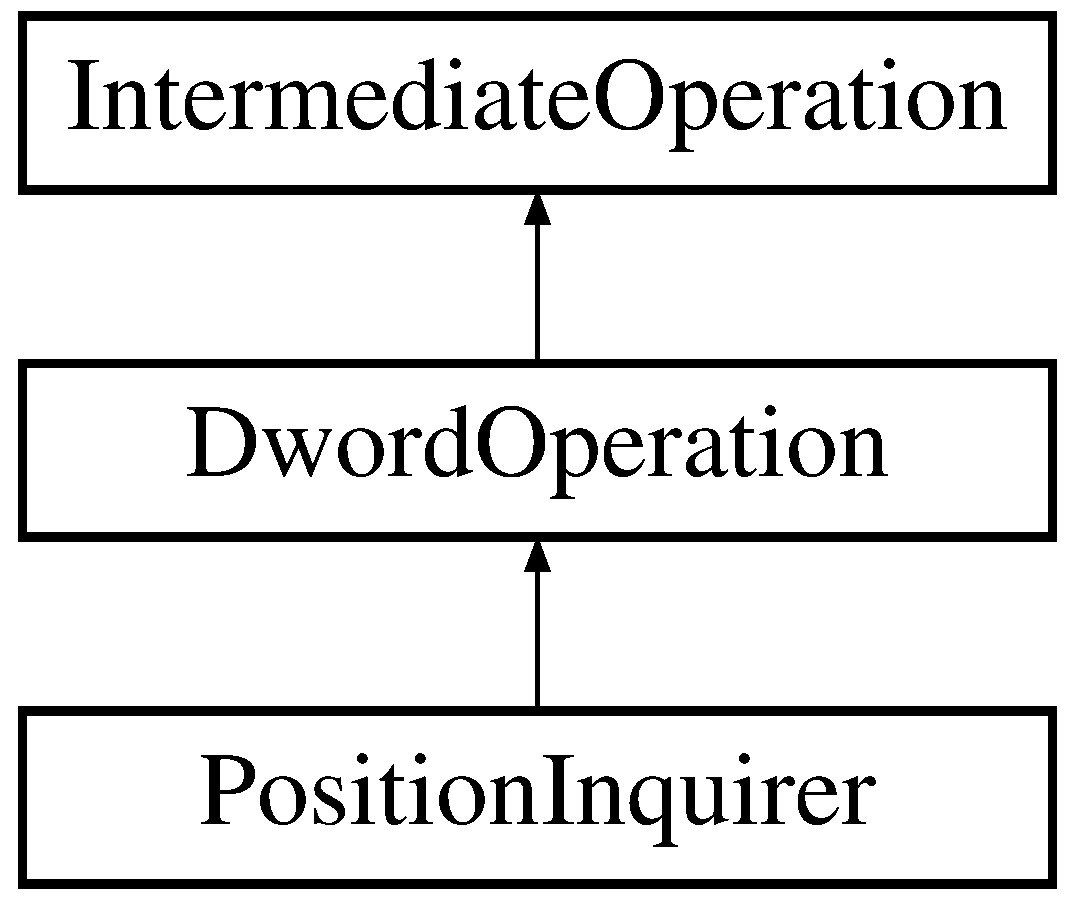
\includegraphics[height=3.000000cm]{d1/d2b/a00018}
\end{center}
\end{figure}
\subsection*{Public Member Functions}
\begin{DoxyCompactItemize}
\item 
\hypertarget{a00018_a0bf888ca94c67257f2c00e7392c8a565}{virtual void {\bfseries provide\+Bytecode} (\hyperlink{a00015}{Operation\+Code} $\ast$a\+Opcode)}\label{a00018_a0bf888ca94c67257f2c00e7392c8a565}

\item 
\hypertarget{a00018_a7218aa1c9025c1763112ac8eb6ebb2fd}{void {\bfseries insert\+Position} (\hyperlink{a00015}{Operation\+Code} $\ast$a\+Opcode, uint a\+Final\+Value)}\label{a00018_a7218aa1c9025c1763112ac8eb6ebb2fd}

\end{DoxyCompactItemize}
\subsection*{Additional Inherited Members}


The documentation for this class was generated from the following files\+:\begin{DoxyCompactItemize}
\item 
E\+:/\+Projects/backup dropbox/\+Scripting/\+Aiki/\+Compiler/Intermediate\+Oper.\+hpp\item 
E\+:/\+Projects/backup dropbox/\+Scripting/\+Aiki/\+Compiler/Intermediate\+Oper.\+cpp\end{DoxyCompactItemize}

\hypertarget{a00019}{\section{Position\+Reference Class Reference}
\label{a00019}\index{Position\+Reference@{Position\+Reference}}
}
Inheritance diagram for Position\+Reference\+:\begin{figure}[H]
\begin{center}
\leavevmode
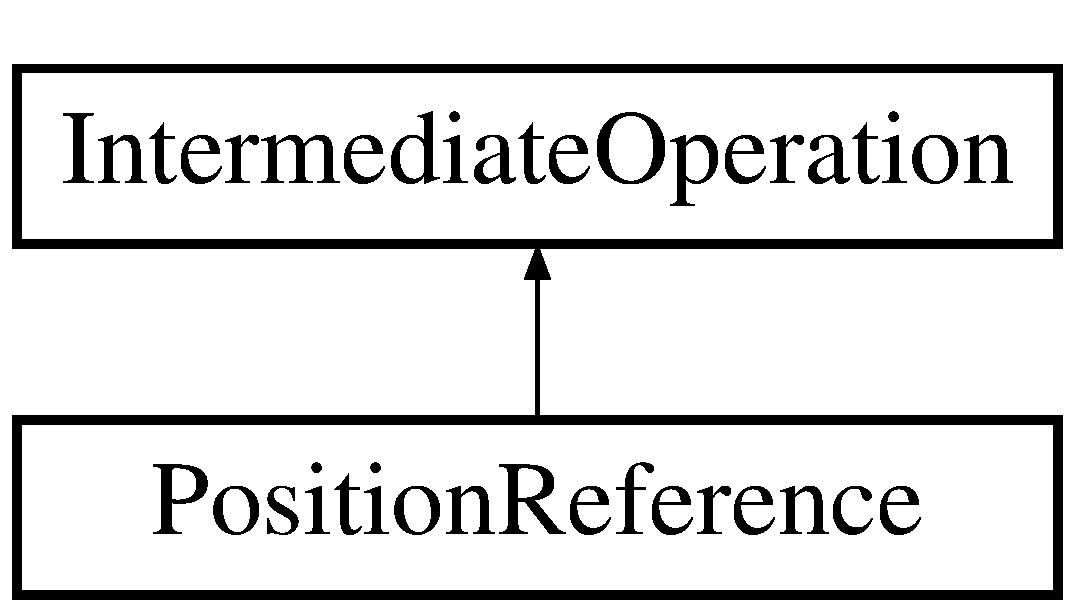
\includegraphics[height=2.000000cm]{dd/da2/a00019}
\end{center}
\end{figure}
\subsection*{Public Member Functions}
\begin{DoxyCompactItemize}
\item 
\hypertarget{a00019_a2238ecbb4faec2237cf7f53faa493251}{void {\bfseries provide\+Bytecode} (\hyperlink{a00015}{Operation\+Code} $\ast$a\+Opcode)}\label{a00019_a2238ecbb4faec2237cf7f53faa493251}

\item 
\hypertarget{a00019_a2ab1c0ad4c5beef59cae0c4de79700d1}{void {\bfseries add\+Inquirer} (\hyperlink{a00018}{Position\+Inquirer} $\ast$a\+Inquirer)}\label{a00019_a2ab1c0ad4c5beef59cae0c4de79700d1}

\end{DoxyCompactItemize}
\subsection*{Protected Attributes}
\begin{DoxyCompactItemize}
\item 
\hypertarget{a00019_a3142d041007ed1ff0606810d07259859}{vector$<$ \hyperlink{a00018}{Position\+Inquirer} $\ast$ $>$ {\bfseries inquirers}}\label{a00019_a3142d041007ed1ff0606810d07259859}

\end{DoxyCompactItemize}


The documentation for this class was generated from the following files\+:\begin{DoxyCompactItemize}
\item 
E\+:/\+Projects/backup dropbox/\+Scripting/\+Aiki/\+Compiler/Intermediate\+Oper.\+hpp\item 
E\+:/\+Projects/backup dropbox/\+Scripting/\+Aiki/\+Compiler/Intermediate\+Oper.\+cpp\end{DoxyCompactItemize}

\hypertarget{a00020}{\section{Return\+Statement Class Reference}
\label{a00020}\index{Return\+Statement@{Return\+Statement}}
}
Inheritance diagram for Return\+Statement\+:\begin{figure}[H]
\begin{center}
\leavevmode
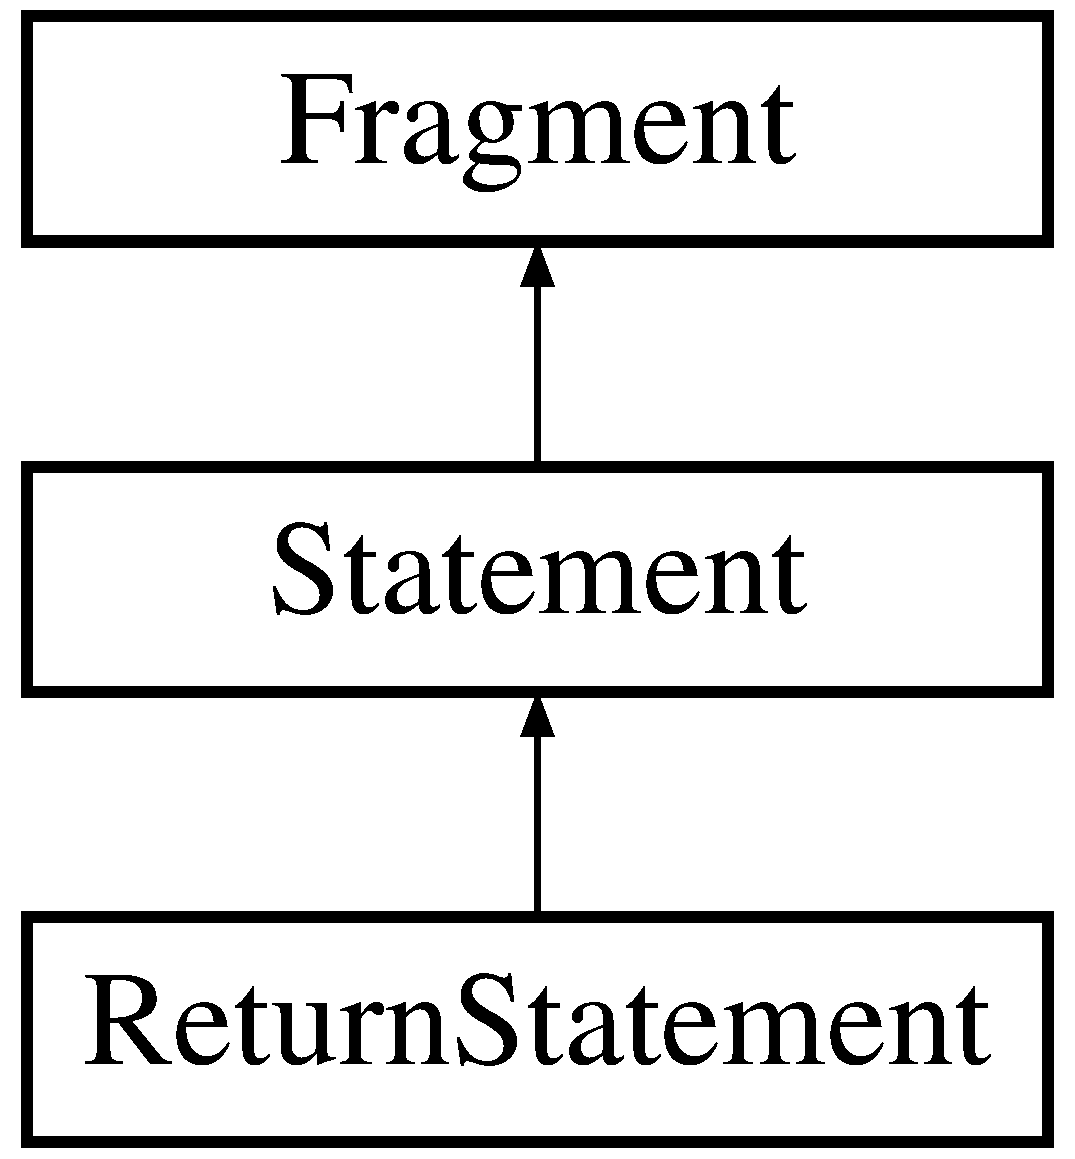
\includegraphics[height=3.000000cm]{db/db2/a00020}
\end{center}
\end{figure}
\subsection*{Public Member Functions}
\begin{DoxyCompactItemize}
\item 
\hypertarget{a00020_a014a69058c260757d442b020db684223}{void {\bfseries parse\+Fragment} (\hyperlink{a00026}{Tokens} $\ast$a\+Tokens, \hyperlink{a00017}{Parser} $\ast$a\+Parser)}\label{a00020_a014a69058c260757d442b020db684223}

\item 
\hypertarget{a00020_a1ef2a1cdad6862bc5d9d18503bc65981}{void {\bfseries provide\+Intermediates} (\hyperlink{a00015}{Operation\+Code} $\ast$a\+Opcode, \hyperlink{a00017}{Parser} $\ast$a\+Parser)}\label{a00020_a1ef2a1cdad6862bc5d9d18503bc65981}

\end{DoxyCompactItemize}
\subsection*{Additional Inherited Members}


The documentation for this class was generated from the following files\+:\begin{DoxyCompactItemize}
\item 
E\+:/\+Projects/backup dropbox/\+Scripting/\+Aiki/\+Compiler/Statement.\+hpp\item 
E\+:/\+Projects/backup dropbox/\+Scripting/\+Aiki/\+Compiler/Statement.\+cpp\end{DoxyCompactItemize}

\hypertarget{a00021}{\section{Scope\+Type$<$ T $>$ Class Template Reference}
\label{a00021}\index{Scope\+Type$<$ T $>$@{Scope\+Type$<$ T $>$}}
}
\subsection*{Public Member Functions}
\begin{DoxyCompactItemize}
\item 
\hypertarget{a00021_a92a1d1964b00c4d0a7af93eaf37c7e93}{uint {\bfseries get\+Item\+I\+D} (T a\+Value)}\label{a00021_a92a1d1964b00c4d0a7af93eaf37c7e93}

\item 
\hypertarget{a00021_a35f343c5c865b3a570f8cfc6e70ee0c2}{bool {\bfseries item\+Exists} (uint a\+I\+D)}\label{a00021_a35f343c5c865b3a570f8cfc6e70ee0c2}

\item 
\hypertarget{a00021_a4f7c5a43069789e9adb9cc1b8d8d95e2}{void {\bfseries add\+Item} (uint id, T t)}\label{a00021_a4f7c5a43069789e9adb9cc1b8d8d95e2}

\item 
\hypertarget{a00021_a3252318a33eb6abc5f6933e7265d4029}{uint {\bfseries get\+Var\+Counter} ()}\label{a00021_a3252318a33eb6abc5f6933e7265d4029}

\item 
\hypertarget{a00021_a3ee6c000d9df265481a508c2a22581a4}{T {\bfseries get\+Var} (uint a\+I\+D)}\label{a00021_a3ee6c000d9df265481a508c2a22581a4}

\item 
\hypertarget{a00021_ae0ca204f4617ce2957de1494c2fe0fd6}{int {\bfseries nest\+Count} ()}\label{a00021_ae0ca204f4617ce2957de1494c2fe0fd6}

\item 
\hypertarget{a00021_a5c8ebe9e5412756c6136e60bbfdf31cb}{void {\bfseries push\+Nested\+Scope} ()}\label{a00021_a5c8ebe9e5412756c6136e60bbfdf31cb}

\item 
\hypertarget{a00021_a8a11c6e96d4f1c29804419d330012582}{void {\bfseries pop\+Nested\+Scope} ()}\label{a00021_a8a11c6e96d4f1c29804419d330012582}

\end{DoxyCompactItemize}
\subsection*{Protected Attributes}
\begin{DoxyCompactItemize}
\item 
\hypertarget{a00021_a553590dc3eebc70ce33fae77071ae56d}{map$<$ uint, T $>$ {\bfseries vars}}\label{a00021_a553590dc3eebc70ce33fae77071ae56d}

\item 
\hypertarget{a00021_a106e1a4efffa0b54e5ef618950eeeb69}{\hyperlink{a00022}{Stack}$<$ \hyperlink{a00021}{Scope\+Type}$<$ T $>$ $\ast$ $>$ {\bfseries joined}}\label{a00021_a106e1a4efffa0b54e5ef618950eeeb69}

\item 
\hypertarget{a00021_acf681b9026dcc2deb745ebeb1baf656a}{uint {\bfseries var\+Counter}}\label{a00021_acf681b9026dcc2deb745ebeb1baf656a}

\end{DoxyCompactItemize}


The documentation for this class was generated from the following file\+:\begin{DoxyCompactItemize}
\item 
E\+:/\+Projects/backup dropbox/\+Scripting/\+Aiki/Scope.\+hpp\end{DoxyCompactItemize}

\hypertarget{a00022}{\section{Stack$<$ T $>$ Class Template Reference}
\label{a00022}\index{Stack$<$ T $>$@{Stack$<$ T $>$}}
}
\subsection*{Public Member Functions}
\begin{DoxyCompactItemize}
\item 
\hypertarget{a00022_abe82b456eaa470780ea183224c47501a}{{\bfseries Stack} (int a\+Max\+Size=2048)}\label{a00022_abe82b456eaa470780ea183224c47501a}

\item 
\hypertarget{a00022_ace28110b50a0a2f4f3c8fd5263413661}{void {\bfseries push} (T val)}\label{a00022_ace28110b50a0a2f4f3c8fd5263413661}

\item 
\hypertarget{a00022_aa2ea0e8c3293648589dd734d52487408}{T {\bfseries pop} ()}\label{a00022_aa2ea0e8c3293648589dd734d52487408}

\item 
\hypertarget{a00022_adcb4774ac8aa94cbc19b461da9bdee3a}{T {\bfseries peek} ()}\label{a00022_adcb4774ac8aa94cbc19b461da9bdee3a}

\item 
\hypertarget{a00022_a753f43c9236116e1e68f52022d24bb3d}{T {\bfseries peek} (int index)}\label{a00022_a753f43c9236116e1e68f52022d24bb3d}

\item 
\hypertarget{a00022_a71b9623c81ddeb690c6fd0c7fb1d7bba}{int {\bfseries Size} ()}\label{a00022_a71b9623c81ddeb690c6fd0c7fb1d7bba}

\end{DoxyCompactItemize}


The documentation for this class was generated from the following file\+:\begin{DoxyCompactItemize}
\item 
E\+:/\+Projects/backup dropbox/\+Scripting/\+Aiki/Stack.\+hpp\end{DoxyCompactItemize}

\hypertarget{a00023}{\section{Statement Class Reference}
\label{a00023}\index{Statement@{Statement}}
}
Inheritance diagram for Statement\+:\begin{figure}[H]
\begin{center}
\leavevmode
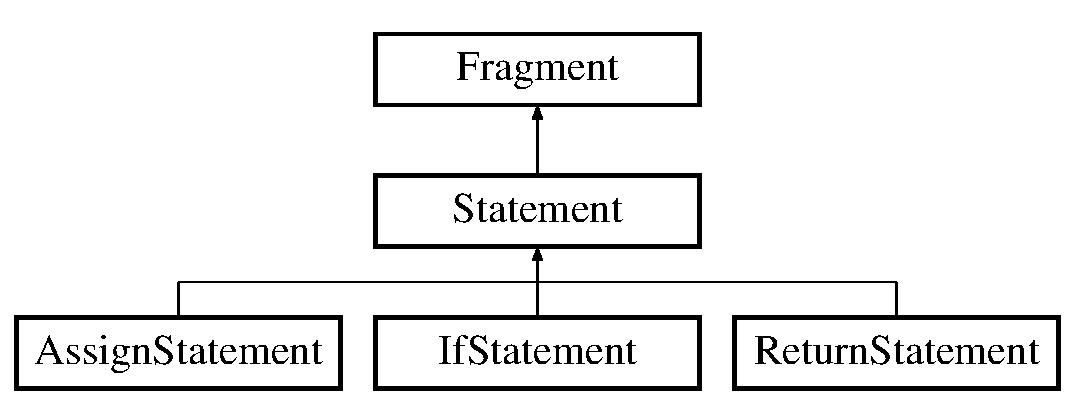
\includegraphics[height=3.000000cm]{d3/d52/a00023}
\end{center}
\end{figure}
\subsection*{Static Public Member Functions}
\begin{DoxyCompactItemize}
\item 
\hypertarget{a00023_a82dcbdec4ea18a7fe7b119b3d75944dc}{static \hyperlink{a00023}{Statement} $\ast$ {\bfseries create\+Statement} (\hyperlink{a00026}{Tokens} $\ast$a\+Tokens, \hyperlink{a00017}{Parser} $\ast$a\+Parser)}\label{a00023_a82dcbdec4ea18a7fe7b119b3d75944dc}

\end{DoxyCompactItemize}
\subsection*{Additional Inherited Members}


The documentation for this class was generated from the following files\+:\begin{DoxyCompactItemize}
\item 
E\+:/\+Projects/backup dropbox/\+Scripting/\+Aiki/\+Compiler/Statement.\+hpp\item 
E\+:/\+Projects/backup dropbox/\+Scripting/\+Aiki/\+Compiler/Statement.\+cpp\end{DoxyCompactItemize}

\hypertarget{a00024}{\section{Aiki\+Std\+:\+:Std\+Func Struct Reference}
\label{a00024}\index{Aiki\+Std\+::\+Std\+Func@{Aiki\+Std\+::\+Std\+Func}}
}
\subsection*{Public Attributes}
\begin{DoxyCompactItemize}
\item 
\hypertarget{a00024_a5edd90a27f903e18328f4d89e63253b6}{int {\bfseries params}}\label{a00024_a5edd90a27f903e18328f4d89e63253b6}

\item 
\hypertarget{a00024_a6d4f1ed3742f29094ab788cf4ba9f86c}{void $\ast$ {\bfseries func}}\label{a00024_a6d4f1ed3742f29094ab788cf4ba9f86c}

\end{DoxyCompactItemize}


The documentation for this struct was generated from the following file\+:\begin{DoxyCompactItemize}
\item 
E\+:/\+Projects/backup dropbox/\+Scripting/\+Aiki/Functions.\+cpp\end{DoxyCompactItemize}

\hypertarget{a00025}{\section{Token Struct Reference}
\label{a00025}\index{Token@{Token}}
}
\subsection*{Public Types}
\begin{DoxyCompactItemize}
\item 
\hypertarget{a00025_acf70e9411196c602738c3ed2428c7137}{enum {\bfseries Type} \{ \\*
{\bfseries I\+N\+V\+A\+L\+I\+D} = 0x80000000, 
{\bfseries U\+N\+D\+E\+F\+I\+N\+E\+D} = 0x00000100, 
{\bfseries O\+P\+E\+R\+A\+T\+O\+R} = 0x00000200, 
{\bfseries O\+P\+E\+R\+A\+T\+O\+R\+\_\+\+A\+R\+I\+T} = 0x00000201, 
\\*
{\bfseries O\+P\+E\+R\+A\+T\+O\+R\+\_\+\+C\+O\+M\+P} = 0x00000202, 
{\bfseries O\+P\+E\+R\+A\+T\+O\+R\+\_\+\+A\+S\+S\+I\+G\+N} = 0x00000204, 
{\bfseries V\+A\+R\+I\+A\+B\+L\+E\+\_\+\+S\+T\+R\+I\+N\+G} = 0x00080000, 
{\bfseries V\+A\+R\+I\+A\+B\+L\+E\+\_\+\+I\+N\+T} = 0x00100000, 
\\*
{\bfseries V\+A\+R\+I\+A\+B\+L\+E\+\_\+\+F\+L\+O\+A\+T} = 0x00200000, 
{\bfseries V\+A\+R\+I\+A\+B\+L\+E\+\_\+\+F\+U\+N\+C\+T\+I\+O\+N} = 0x00400000, 
{\bfseries P\+A\+R\+A\+N\+T\+H\+\_\+\+B\+E\+G} = 0x00000400, 
{\bfseries P\+A\+R\+A\+N\+T\+H\+\_\+\+E\+N\+D} = 0x00000800, 
\\*
{\bfseries R\+E\+S\+E\+R\+V\+E\+D} = 0x00001000, 
{\bfseries B\+R\+A\+C\+K\+E\+T\+\_\+\+B\+E\+G} = 0x00002000, 
{\bfseries B\+R\+A\+C\+K\+E\+T\+\_\+\+E\+N\+D} = 0x00004000, 
{\bfseries V\+A\+L\+U\+E} = 0x00040000, 
\\*
{\bfseries S\+E\+M\+I\+C\+O\+L\+O\+N} = 0x00008000, 
{\bfseries D\+O\+T} = 0x00010000, 
{\bfseries C\+O\+M\+M\+A} = 0x00020000
 \}}\label{a00025_acf70e9411196c602738c3ed2428c7137}

\end{DoxyCompactItemize}
\subsection*{Public Member Functions}
\begin{DoxyCompactItemize}
\item 
\hypertarget{a00025_a440f7c33c975cc2bd14dfed35ab3fcea}{{\bfseries Token} (std\+::string a\+Token, Type t=I\+N\+V\+A\+L\+I\+D)}\label{a00025_a440f7c33c975cc2bd14dfed35ab3fcea}

\end{DoxyCompactItemize}
\subsection*{Static Public Member Functions}
\begin{DoxyCompactItemize}
\item 
\hypertarget{a00025_ae6f28995197884ebeb2e22989a193a44}{static std\+::string {\bfseries get\+String\+Value} (Token\+::\+Type a\+Type)}\label{a00025_ae6f28995197884ebeb2e22989a193a44}

\end{DoxyCompactItemize}
\subsection*{Public Attributes}
\begin{DoxyCompactItemize}
\item 
\hypertarget{a00025_a290d52d875142e4728d4c23e1be7e316}{std\+::string {\bfseries token}}\label{a00025_a290d52d875142e4728d4c23e1be7e316}

\item 
\hypertarget{a00025_a8be912d99c08d7ac8669552abfd1392b}{Type {\bfseries a\+Type}}\label{a00025_a8be912d99c08d7ac8669552abfd1392b}

\end{DoxyCompactItemize}


The documentation for this struct was generated from the following files\+:\begin{DoxyCompactItemize}
\item 
E\+:/\+Projects/backup dropbox/\+Scripting/\+Aiki/\+Compiler/Tokens.\+hpp\item 
E\+:/\+Projects/backup dropbox/\+Scripting/\+Aiki/\+Compiler/Tokens.\+cpp\end{DoxyCompactItemize}

\hypertarget{a00026}{\section{Tokens Class Reference}
\label{a00026}\index{Tokens@{Tokens}}
}
\subsection*{Public Member Functions}
\begin{DoxyCompactItemize}
\item 
\hypertarget{a00026_a60ba2f31bd640b06347b2b05e0c49bce}{void {\bfseries generate\+Tokens} (std\+::string a\+File)}\label{a00026_a60ba2f31bd640b06347b2b05e0c49bce}

\item 
\hypertarget{a00026_a3937c350677be513f8fae9bb039b5048}{void {\bfseries set\+Pointer} (Token\+Iterertor a\+Front)}\label{a00026_a3937c350677be513f8fae9bb039b5048}

\item 
\hypertarget{a00026_ac77fef2bf79930113c4a0ee184574924}{\hyperlink{a00025}{Token} $\ast$ {\bfseries pop\+If\+Exists} (Token\+::\+Type a\+Type)}\label{a00026_ac77fef2bf79930113c4a0ee184574924}

\item 
\hypertarget{a00026_a9c3df0010d1c782ac84e8124d8b504d6}{\hyperlink{a00025}{Token} $\ast$ {\bfseries pop\+Expected} (Token\+::\+Type a\+Type)}\label{a00026_a9c3df0010d1c782ac84e8124d8b504d6}

\item 
\hypertarget{a00026_a25d0c3de304ab05f23855c512e8e15f6}{\hyperlink{a00025}{Token} $\ast$ {\bfseries pop\+Next} ()}\label{a00026_a25d0c3de304ab05f23855c512e8e15f6}

\item 
\hypertarget{a00026_a1b7b5a9cc72ab57874c90ab8feb10934}{\hyperlink{a00025}{Token} $\ast$ {\bfseries check\+Next} ()}\label{a00026_a1b7b5a9cc72ab57874c90ab8feb10934}

\item 
\hypertarget{a00026_a4cb230238fa3fa1ac0586b8289b3b666}{Token\+Iterertor {\bfseries get\+First\+Iterator} ()}\label{a00026_a4cb230238fa3fa1ac0586b8289b3b666}

\item 
\hypertarget{a00026_ab35f81cfa85c12e184ead391d4c6bdbd}{Token\+Iterertor {\bfseries get\+Pointer} ()}\label{a00026_ab35f81cfa85c12e184ead391d4c6bdbd}

\item 
\hypertarget{a00026_a9531391ac07caf1f8df162d7e2660b62}{bool {\bfseries is\+More} ()}\label{a00026_a9531391ac07caf1f8df162d7e2660b62}

\end{DoxyCompactItemize}


The documentation for this class was generated from the following files\+:\begin{DoxyCompactItemize}
\item 
E\+:/\+Projects/backup dropbox/\+Scripting/\+Aiki/\+Compiler/Tokens.\+hpp\item 
E\+:/\+Projects/backup dropbox/\+Scripting/\+Aiki/\+Compiler/Tokens.\+cpp\end{DoxyCompactItemize}

\hypertarget{a00027}{\section{Variable Class Reference}
\label{a00027}\index{Variable@{Variable}}
}
\subsection*{Public Types}
\begin{DoxyCompactItemize}
\item 
\hypertarget{a00027_a132ec67f164061bacffc204425dc1eb1}{enum {\bfseries Type} \{ \\*
{\bfseries U\+N\+D\+E\+F\+I\+N\+E\+D}, 
{\bfseries I\+N\+T}, 
{\bfseries F\+L\+O\+A\+T}, 
{\bfseries S\+T\+R\+I\+N\+G}, 
\\*
{\bfseries O\+B\+J\+E\+C\+T}
 \}}\label{a00027_a132ec67f164061bacffc204425dc1eb1}

\end{DoxyCompactItemize}
\subsection*{Public Member Functions}
\begin{DoxyCompactItemize}
\item 
\hypertarget{a00027_a85762c842cb279744763a3d987d0220a}{{\bfseries Variable} (int a\+I\+D=0)}\label{a00027_a85762c842cb279744763a3d987d0220a}

\item 
\hypertarget{a00027_a5a4ba3b52af5668064d2cc4a14dfbd39}{Type {\bfseries get\+Type} () const }\label{a00027_a5a4ba3b52af5668064d2cc4a14dfbd39}

\item 
\hypertarget{a00027_add84de4a866b07c8ce12d5ba437c1177}{int {\bfseries get\+I\+D} () const }\label{a00027_add84de4a866b07c8ce12d5ba437c1177}

\item 
\hypertarget{a00027_a96541cad47a888a3faf5ac95ebb642c1}{int {\bfseries get\+Integer} () const }\label{a00027_a96541cad47a888a3faf5ac95ebb642c1}

\item 
\hypertarget{a00027_accd18c593f68e10f4960d3f2da4cef3e}{float {\bfseries get\+Float} () const }\label{a00027_accd18c593f68e10f4960d3f2da4cef3e}

\item 
\hypertarget{a00027_a8d777ed20b189d668564586e08794a3b}{const char $\ast$ {\bfseries get\+String} () const }\label{a00027_a8d777ed20b189d668564586e08794a3b}

\item 
\hypertarget{a00027_ade1810d281d0573dc61aa40b2a26bd4f}{void {\bfseries set} (int)}\label{a00027_ade1810d281d0573dc61aa40b2a26bd4f}

\item 
\hypertarget{a00027_a2f1bafa54a211691509471177b054ec4}{void {\bfseries set} (float)}\label{a00027_a2f1bafa54a211691509471177b054ec4}

\item 
\hypertarget{a00027_a70c43bd069987bc4bebd9b586c6688f2}{void {\bfseries set} (const char $\ast$)}\label{a00027_a70c43bd069987bc4bebd9b586c6688f2}

\item 
\hypertarget{a00027_a89d980fdc6a07075624598e58a9ee420}{void {\bfseries undefine} ()}\label{a00027_a89d980fdc6a07075624598e58a9ee420}

\item 
\hypertarget{a00027_afe7599538dad80403536f47710588b0f}{void {\bfseries operator=} (const \hyperlink{a00027}{Variable} \&a\+Variable)}\label{a00027_afe7599538dad80403536f47710588b0f}

\item 
\hypertarget{a00027_a7aa8b9995152f962c251fbcbff28399b}{void {\bfseries operator+=} (const \hyperlink{a00027}{Variable} \&a\+Variable)}\label{a00027_a7aa8b9995152f962c251fbcbff28399b}

\item 
\hypertarget{a00027_a14f76c8a893def148e3d45a07ef3a227}{void {\bfseries operator+=} (const int \&a\+Variable)}\label{a00027_a14f76c8a893def148e3d45a07ef3a227}

\item 
\hypertarget{a00027_aa15ad843f92054866a5b91661ad9aeb7}{void {\bfseries operator+=} (const float \&a\+Variable)}\label{a00027_aa15ad843f92054866a5b91661ad9aeb7}

\item 
\hypertarget{a00027_aff91cecf748f1c578f65390b8c1d3611}{void {\bfseries operator-\/=} (const \hyperlink{a00027}{Variable} \&a\+Variable)}\label{a00027_aff91cecf748f1c578f65390b8c1d3611}

\item 
\hypertarget{a00027_a7f6a8376fbc35ca758627ba11288e7a9}{void {\bfseries operator-\/=} (const int \&a\+Variable)}\label{a00027_a7f6a8376fbc35ca758627ba11288e7a9}

\item 
\hypertarget{a00027_ac50b02bdeb91289cb2f30c8561a659c9}{void {\bfseries operator-\/=} (const float \&a\+Variable)}\label{a00027_ac50b02bdeb91289cb2f30c8561a659c9}

\item 
\hypertarget{a00027_a3bd38cc163ab6c908d110b1cd468a035}{void {\bfseries operator$\ast$=} (const \hyperlink{a00027}{Variable} \&a\+Variable)}\label{a00027_a3bd38cc163ab6c908d110b1cd468a035}

\item 
\hypertarget{a00027_aca6bbd6730eed87adf4fa23810c3eee1}{void {\bfseries operator$\ast$=} (const int \&a\+Variable)}\label{a00027_aca6bbd6730eed87adf4fa23810c3eee1}

\item 
\hypertarget{a00027_aa7dd21e6d4bcb73d4cf659e10d062f44}{void {\bfseries operator$\ast$=} (const float \&a\+Variable)}\label{a00027_aa7dd21e6d4bcb73d4cf659e10d062f44}

\item 
\hypertarget{a00027_a8ac9083e343d9345fff3c5faaf8571e3}{void {\bfseries operator/=} (const \hyperlink{a00027}{Variable} \&a\+Variable)}\label{a00027_a8ac9083e343d9345fff3c5faaf8571e3}

\item 
\hypertarget{a00027_a44a8a5fea30597cc3a5c81715fb5babc}{void {\bfseries operator/=} (const int \&a\+Variable)}\label{a00027_a44a8a5fea30597cc3a5c81715fb5babc}

\item 
\hypertarget{a00027_abcb80a08c60c33570933c89214684028}{void {\bfseries operator/=} (const float \&a\+Variable)}\label{a00027_abcb80a08c60c33570933c89214684028}

\item 
\hypertarget{a00027_a4bd7a3b7aa71b11670fcf8e296cf0fdf}{void {\bfseries operator\%=} (const \hyperlink{a00027}{Variable} \&a\+Variable)}\label{a00027_a4bd7a3b7aa71b11670fcf8e296cf0fdf}

\item 
\hypertarget{a00027_a627ab13fe2bd0eb446e5ae375fa38fa4}{void {\bfseries operator\%=} (const int \&a\+Variable)}\label{a00027_a627ab13fe2bd0eb446e5ae375fa38fa4}

\item 
\hypertarget{a00027_acba93d650c9836d3e9c8cff9187fe796}{bool {\bfseries operator$>$} (const \hyperlink{a00027}{Variable} \&a\+Variable) const }\label{a00027_acba93d650c9836d3e9c8cff9187fe796}

\item 
\hypertarget{a00027_af08d02bb113bb86dd834fa4d8dd2f1c6}{bool {\bfseries operator$>$} (const int \&a\+Variable) const }\label{a00027_af08d02bb113bb86dd834fa4d8dd2f1c6}

\item 
\hypertarget{a00027_a9f41035d7fe454337e150f17ec82a7d8}{bool {\bfseries operator$>$} (const float \&a\+Variable) const }\label{a00027_a9f41035d7fe454337e150f17ec82a7d8}

\item 
\hypertarget{a00027_a8b9805a6248f2ae3628a130bdbefa7d4}{bool {\bfseries operator$>$=} (const \hyperlink{a00027}{Variable} \&a\+Variable) const }\label{a00027_a8b9805a6248f2ae3628a130bdbefa7d4}

\item 
\hypertarget{a00027_a7039b8a279eda6c99d05e30a5cf8d52f}{bool {\bfseries operator$>$=} (const int \&a\+Variable) const }\label{a00027_a7039b8a279eda6c99d05e30a5cf8d52f}

\item 
\hypertarget{a00027_aec9f1b2fb385976327e945df5713b75c}{bool {\bfseries operator$>$=} (const float \&a\+Variable) const }\label{a00027_aec9f1b2fb385976327e945df5713b75c}

\item 
\hypertarget{a00027_ab3f60f12efcd38436379ca2e94503e97}{bool {\bfseries operator$<$} (const \hyperlink{a00027}{Variable} \&a\+Variable) const }\label{a00027_ab3f60f12efcd38436379ca2e94503e97}

\item 
\hypertarget{a00027_a7128a2f9884ba7222e9f208cf72687bf}{bool {\bfseries operator$<$} (const int \&a\+Variable) const }\label{a00027_a7128a2f9884ba7222e9f208cf72687bf}

\item 
\hypertarget{a00027_a5ab2b61d4607368b6f14a50684d1ecfe}{bool {\bfseries operator$<$} (const float \&a\+Variable) const }\label{a00027_a5ab2b61d4607368b6f14a50684d1ecfe}

\item 
\hypertarget{a00027_aacb11a665a3e9552980747e6d842162d}{bool {\bfseries operator$<$=} (const \hyperlink{a00027}{Variable} \&a\+Variable) const }\label{a00027_aacb11a665a3e9552980747e6d842162d}

\item 
\hypertarget{a00027_a7ac8de58557d03d71305e126f8a956a5}{bool {\bfseries operator$<$=} (const int \&a\+Variable) const }\label{a00027_a7ac8de58557d03d71305e126f8a956a5}

\item 
\hypertarget{a00027_a5aa6c62d3f1fcd234b91583840de4be4}{bool {\bfseries operator$<$=} (const float \&a\+Variable) const }\label{a00027_a5aa6c62d3f1fcd234b91583840de4be4}

\item 
\hypertarget{a00027_adf8d943c0ffb988e6c3ca02f6655bd0c}{bool {\bfseries operator==} (const \hyperlink{a00027}{Variable} \&a\+Variable) const }\label{a00027_adf8d943c0ffb988e6c3ca02f6655bd0c}

\item 
\hypertarget{a00027_a38b9c17962d150167df81278f078cd8f}{bool {\bfseries operator==} (const int \&a\+Variable) const }\label{a00027_a38b9c17962d150167df81278f078cd8f}

\item 
\hypertarget{a00027_afa901b4271c8e247067b58e7f13db143}{bool {\bfseries operator==} (const float \&a\+Variable) const }\label{a00027_afa901b4271c8e247067b58e7f13db143}

\item 
\hypertarget{a00027_aade291dab2de60dbd5413599b1a816a4}{bool {\bfseries operator!=} (const \hyperlink{a00027}{Variable} \&a\+Variable) const }\label{a00027_aade291dab2de60dbd5413599b1a816a4}

\item 
\hypertarget{a00027_a849761ed0d493ff8c341d85ee77f3ad1}{bool {\bfseries operator!=} (const int \&a\+Variable) const }\label{a00027_a849761ed0d493ff8c341d85ee77f3ad1}

\item 
\hypertarget{a00027_aac4ceb266a19c0f3dd456f01ca6a9961}{bool {\bfseries operator!=} (const float \&a\+Variable) const }\label{a00027_aac4ceb266a19c0f3dd456f01ca6a9961}

\end{DoxyCompactItemize}
\subsection*{Static Public Member Functions}
\begin{DoxyCompactItemize}
\item 
\hypertarget{a00027_a6f6b6ddbc721a4a702473a145e862a1b}{static \hyperlink{a00027}{Variable} $\ast$ {\bfseries create\+Variable} (const char $\ast$a\+Value)}\label{a00027_a6f6b6ddbc721a4a702473a145e862a1b}

\item 
\hypertarget{a00027_a0c78560da5419d9096e09dd562932735}{static Type {\bfseries get\+Type} (std\+::string a\+String)}\label{a00027_a0c78560da5419d9096e09dd562932735}

\end{DoxyCompactItemize}


The documentation for this class was generated from the following files\+:\begin{DoxyCompactItemize}
\item 
E\+:/\+Projects/backup dropbox/\+Scripting/\+Aiki/\+Parser/Variable.\+hpp\item 
E\+:/\+Projects/backup dropbox/\+Scripting/\+Aiki/\+Parser/Variable.\+cpp\end{DoxyCompactItemize}

%--- End generated contents ---

% Index
\newpage
\phantomsection
\addcontentsline{toc}{chapter}{Index}
\printindex

\end{document}
